%*******************************************************************************
%****************************** Fifth Chapter *********************************
%*******************************************************************************

\chapter{Cosmic $\mu$ Tomography}\label{chp:cosmicMuTelescopes}

\ifpdf
    \graphicspath{{Chapter5/Figs/Raster/}{Chapter5/Figs/PDF/}{Chapter5/Figs/}}
\else
    \graphicspath{{Chapter5/Figs/Vector/}{Chapter5/Figs/}}
\fi

% In spherical polar coordinates, there is also a polar angle commonly denoted as $\theta$. Figure \ref{fig:sphericalPolarCoordinateSystem} shows the coordinate system in $\phi$ and $\theta$ being used

% This chapter is an overview of cosmic $\mu$ tomography and an overview of the MU-RAY and DIAPHANE detectors. It will cover the techniques that both collaborations use and why the ``transmission'' technique from the MU-RAY collaboration is especially valuable.

Due to COVID-19 pandemic the focus of the Ph.D. had to change, the upgrade stalled as global supply chains failed. Therefore, the old data set taken by RMon at Wylfa was reopened and cosmic $\mu$ tomography was attempted. But first the topic of cosmic $\mu$ tomography needs to be well understood and in this chapter an overview of cosmic $\mu$ tomography follows. In this chapter there will be an overview of cosmic $\mu$ tomography. This includes the production of cosmic $\mu$ in the atmosphere and various fields that use tomography. In general there are two distinct forms of cosmic $\mu$ tomography, two-sided, and one-sided their advantages and disadvantages will will be discussed here. In addition, three main applications of tomography will be considered here as well, two-sided reactor tomography, one-sided reactor tomography, and one-sided geological tomography.

\section{Production Of Cosmic $\mu$ In The Atmosphere} 
Atmospheric $\mu$ are produced when high energy protons interact with nuclei in the atmosphere \cite{griffiths2008neutrinoOscillations}. An example of a cosmic shower can be seen in figure \ref{fig:muonShower}, which shows how the production of $\pi^+$ and $\pi^-$ from the initial proton interaction leads to the production of $\mu^-$ and $\mu^+$ particles (equation \ref{equ:pi+-atmos}) \cite{griffiths2008neutrinoOscillations}. There are three main sources of cosmic protons: solar, Galactic, and extra-Galactic \cite{Drury2012OCosmicRays} \cite{muscheler2013_10be} \cite{Pierre2017Aniostropy}. Extra-Galactic particles are rare and typically have high energies of $\sim$ 10$^{18}$\,eV \cite{Pierre2017Aniostropy}. Whilst during specific short term events the number of solar cosmic rays penetrating the atmosphere can be several orders of magnitude higher than the flux of Galactic cosmic rays the energy of solar events is much lower than the Galactic events \cite{muscheler2013_10be}. In general, cosmic rays observed at mildly relativistic energies, around 1\,GeV per nucleon are of exclusively Galactic origin \cite{Drury2012OCosmicRays}. Supernovae are considered to be the main source of Galactic cosmic rays as they are the most viable candidates to produce particles with such energy \cite{Drury2012OCosmicRays}. Typically the kinetic energy for $\mu^-$ and $\mu^+$ is $\sim$ 4\,GeV in the atmosphere \cite{MuonPhysics} \cite{ieee_cry_2007}. Therefore, for most cosmic rays it is reasonable to assume Galactic origin, and as such the onset of night at any given site may have little effect on cosmic $\mu$ production. Typically these cosmic $\mu$ are treated as noise and are often characterised to gain an understanding of their contribution to the background. For example, his was done during the author's 6 month placement at A.W.E (see appendix \ref{appen:AweReportOnCosmicMu})\footnote{Appendix \ref{appen:AweReportOnCosmicMu} is a casual internal report designed to explain the work to a hand-off scientist it is not written to the same standard as this thesis.}.

\begin{figure}[!h]
 \centering
 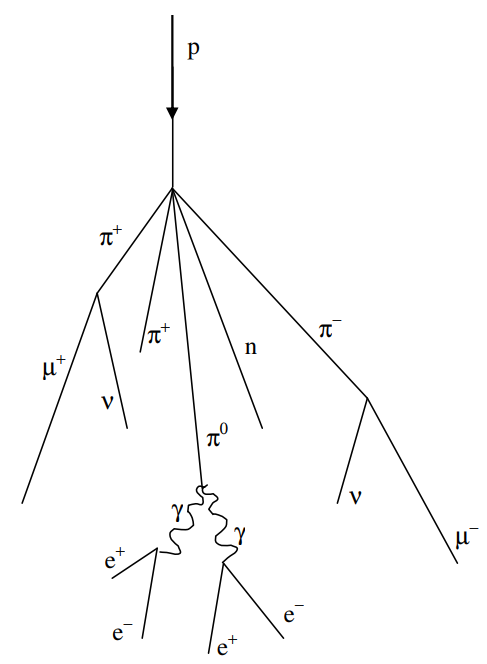
\includegraphics[width=0.3333\linewidth]{Chapter5/Figs/Raster/muonShower.png}
 \captionof{figure}{An illustration of the shower of particles produced by cosmic ray collisions. Atmospheric $\mu$ are produced from the secondary $\pi^+$ and $\pi^-$ in the atmosphere which are in turn produced from hadronic collisions with protons and atmospheric nuclei. From \cite{MuonPhysics}.}
 \label{fig:muonShower}
\end{figure}

\begin{equation}
  \pi^+ \rightarrow \mu^+ + \nu_\mu  \qquad \qquad \pi^- \rightarrow \mu^- + \Bar{\nu_\mu} 
  \label{equ:pi+-atmos}
\end{equation}

\section{Overview Of Cosmic $\mu$ Tomography}\label{sec:cosMuOverview}
%What is cosmic muon tomography? What does the process include? 
%Whats the difference between muon tomography and muon radiography?
The principle novelty of cosmic muon tomography is the ability to measure the angles of arriving cosmic ray $\mu$ with great precision over a sensitive area \cite{Alvarez_Pyramids_1970}. One of the first and most notable uses for cosmic $\mu$ tomography was imaging the second pyramid of Giza in 1970 \cite{Alvarez_Pyramids_1970}. One of the major concerns surrounding cosmic $\mu$ tomography was and still is the amount of scattering caused from measuring high z materials \cite{Alvarez_Pyramids_1970}. Cosmic $\mu$ tomography requires the use of precise instrumentation to accurately resolve the incoming particles. For example, the advent of spark chambers was required for pyramid imaging \cite{Alvarez_Pyramids_1970}. 
\\\\Cosmic $\mu$ tomography allows for positional reconstruction of a detectors surroundings. This positional reconstruction is useful because it guards against the detector from being forcibly relocated. $\Bar{\nu_e}$ cannot be obscured due to their small cross section of 10$^{-42}$\,cm$^2$. As a result the only method to deceive an $\Bar{\nu_e}$ detector (bar tampering) is to relocate it. GPS trackers are a solution but can be potentially jammed therefore positional guarding via cosmic $\mu$ tomography is desirable. Considering the length of time to cycle power in reactors and thus remove fuel and by extension weapons grade material a time of 1\,hour was targeted to build sufficient statistics whilst being unobtrusive to $\Bar{\nu_e}$ reactor monitoring. Fortunately cosmic $\mu$ events were taken in accidental coincidence during the Wylfa deployment this afforded a fantastic opportunity to test the tomographic capabilities of the detector. To that end an overview of other detectors will follow to asses the limitations of this approach. 
\\\\Cosmic $\mu$ tomography can be split into two distinct types: two-sided cosmic $\mu$ tomography measures the incoming $\mu$ angles and outgoing $\mu$ angles over a given area with an object of interest to be imaged as shown by figure \ref{fig:twoSidedCosmicMuonTomographySchults}. This approach allows for vertex reconstruction and measures cosmic $\mu$ scattering thus giving a detailed interior image of the object being imaged \cite{schultz_2007}. This approach has been used to analyse nuclear waste \cite{jonkmans2013nuclear} and even imaging the Fukushima Daiichi reactors \cite{miyadera2013imaging}. However, as figure \ref{fig:twoSidedCosmicMuonTomographySchults} shows the  detectors are typically much larger or of similar size to the object that they are attempting to image. So whilst this technique would yield a very accurate breakdown of the internal structure of any given object it would not be suitable in all cases. For example, if an object of interest is much larger than the detector only a small portion of it can be analysed. 

\begin{figure}[!h]
 \centering
 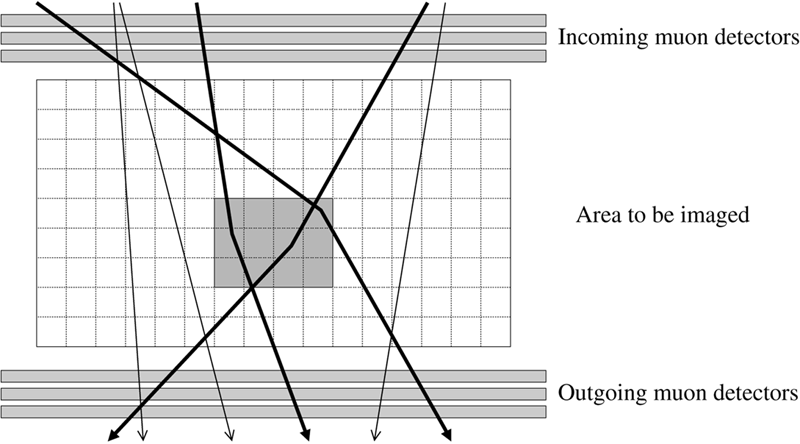
\includegraphics[width=0.7\linewidth]{Chapter5/Figs/Raster/twoSidedCosmicMuon_schults2007.png}
 \captionof{figure}{A side-on view of two-sided cosmic $\mu$ tomography the detectors are of similar size or larger than the object that is being measured in order to make coincided measurements using cosmic $\mu$ seen in the scattered (black) cosmic $\mu$. From \cite{schultz_2007}.}
 \label{fig:twoSidedCosmicMuonTomographySchults}
\end{figure}
 
%  \begin{figure}[!h]
%  \centering
%  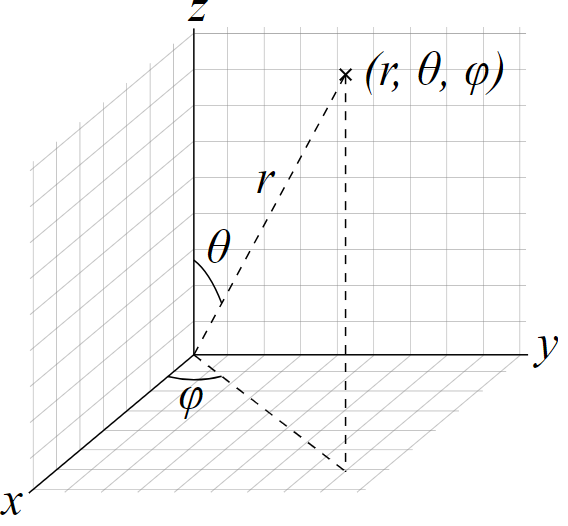
\includegraphics[width=0.3\linewidth]{Chapter5/Figs/wylfaRasterNew/sphericalPolarCoordinatesystem.png}
%  \captionof{figure}{The spherical polar coordinate system is typically used in physics with the azimuthal angle denoted by $\phi$ and the polar angle denoted by $\theta$. Taken from Wikipedia \cite{wikipeidaSphericalCoordinateSystem}.} 
%  \label{fig:sphericalPolarCoordinateSystem}
% \end{figure}
 
 One-sided cosmic $\mu$ tomography is where one detector is used to measure the cosmic $\mu$ incidence, a simplistic example can be seen in figure \ref{subFig:TopDownCircularWallPlot}. Figure \ref{subFig:TopDownCircularWallPlot} is an extremely simplified case where there is a singular wall that blocks 50\,\% of cosmic $\mu$ incidence. However, such a scenario is unlikely except for extremely high Z materials \cite{schultz_2007}. A more realistic example would be in figure \ref{subFig:TopDownCircularCubePlot} where the increasing amount of material corresponds with a decreasing attenuation producing a curve shape in the occluded angles of $\phi$. The top-down perspective in figures \ref{subFig:TopDownCircularWallPlot} and \ref{subFig:TopDownCircularCubePlot} only show the azimuthal angle ($\phi$). If figure \ref{subFig:TopDownCircularCubePlot} is taken and analysed in both $\phi$ and $\theta$ a 360$^\circ$ panoramic view is produced (figure \ref{fig:thetaVsPhiExpectedCube}). 
 
 \begin{figure}[!h]
\centering
\begin{subfigure}{.5\textwidth}
  \centering
  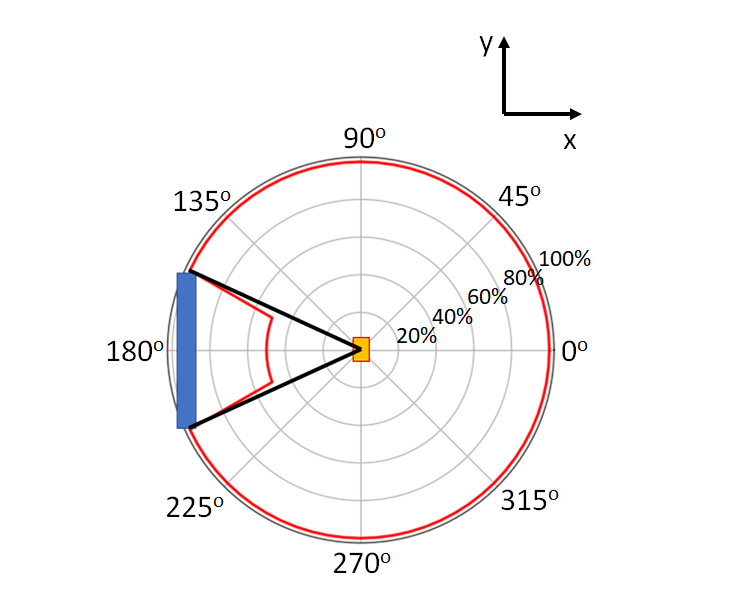
\includegraphics[width=\linewidth]{Chapter5/Figs/topDownWallPhiRedo.png}
  \captionsetup{width=.9\linewidth}
  \caption{}
  \label{subFig:TopDownCircularWallPlot}
\end{subfigure}%
\begin{subfigure}{.5\textwidth}
  \centering
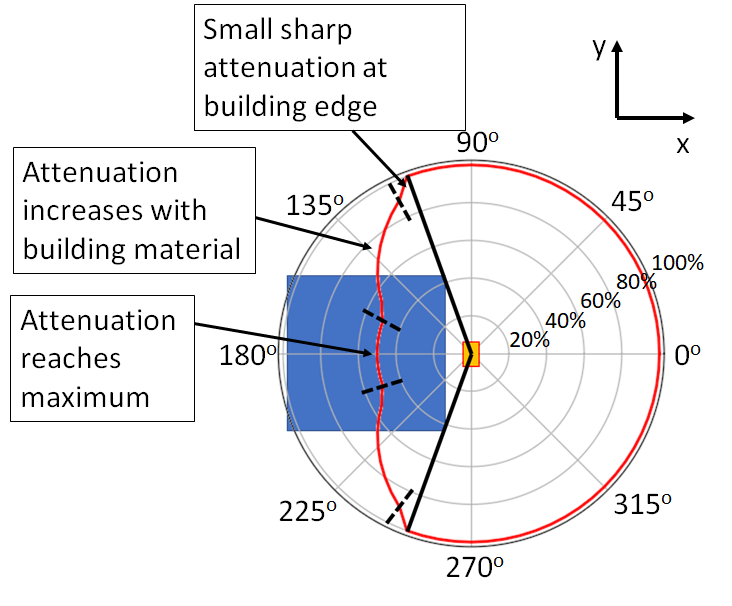
\includegraphics[width=\linewidth]{Chapter5/Figs/topDownCubePhiRedo.png}
  \captionsetup{width=.9\linewidth}
  \caption{}
  \label{subFig:TopDownCircularCubePlot}
\end{subfigure}
\caption{(a) A thin dense wall that blocks 50\,\% of cosmic $\mu$ incidence would look from a top-down perspective. A sharp drop in incidence at the edges with no further attenuation. (b) How a cube of material would block cosmic $\mu$ incidence from a top-down perspective. The amount of attenuation corresponds to the amount of material in the path of the cosmic $\mu$.}
\label{fig:TopDownCircularWallCubePlot}
\end{figure}
 
 \begin{figure}[!h]
 \centering
 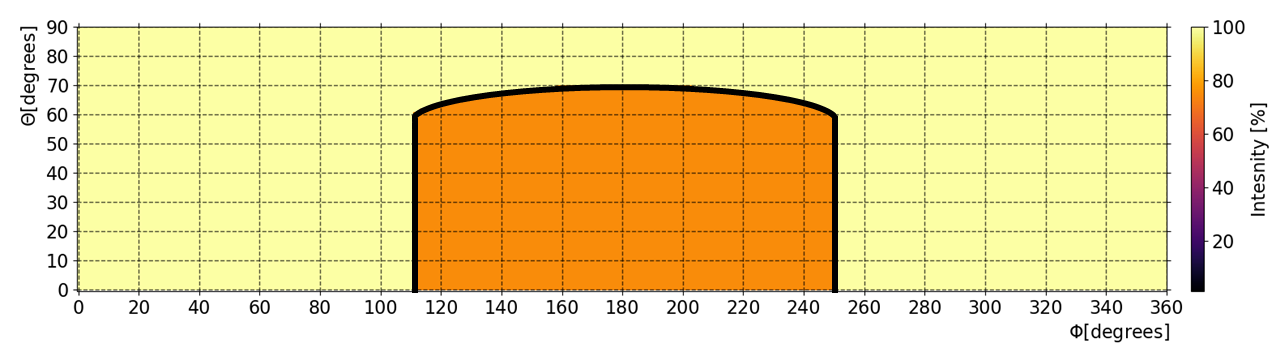
\includegraphics[width=\linewidth]{Chapter5/Figs/wylfaRasterNew/phiVsThetaExpectedInferno_outlined.png}
 \captionof{figure}{How the example seen in figure \ref{subFig:TopDownCircularCubePlot} can be represented in $\theta$ and $\phi$. Assuming it's a cuboid.} 
 \label{fig:thetaVsPhiExpectedCube}
\end{figure}

For figure \ref{fig:thetaVsPhiExpectedCube} there is a slight distortion caused at the top of the building due to the projection of a hemispherical distribution onto a cuboid detector. The amount of distortion will also vary depending on the distance from the detector and the size and shape of the building in question. Longer shorter buildings will have significantly than tall narrow buildings. The slope of the distortion will also vary depending on the position relative to the detector. Further, in figure \ref{fig:thetaVsPhiExpectedCube} the drop in intensity would not be expected to be instantaneous, there would be a gradual decrease in intensity resulting in blurred edges around the occlusion pattern or ``shadow.'' These effects will vary depending on the setup. The VIDARR detector for example is a cuboid detector that analyses the whole hemisphere at once, and as such can be considered as 360$^\circ$ cosmic camera rather than as a cosmic $\mu$ telescope in the strictest sense. This is an important consideration as the other cosmic $\mu$ experiments have very different experimental setups. As will be seen in section \ref{sec:muTomographyExamples}.

\section{$\mu$ Tomography Examples} \label{sec:muTomographyExamples}
There are several fields that utilise cosmic $\mu$ tomography. These include archaeology, geological physics, reactor imaging, and nuclear waste imaging. Archaeology requires a large man made structure with potentially hidden rooms, and so is a niche application \cite{Alvarez_Pyramids_1970}. Nuclear waste imaging utilises two-sided cosmic $\mu$ tomography to ascertain detailed information \cite{jonkmans2013nuclear}. Two-sided reactor tomography is also used for reactor monitoring as the extra information afforded by two-sided tomography is highly desirable \cite{miyadera2013imaging} \cite{perry_imaging_2013} \cite{morris2014analysis}. Though the simplicity and ease of deployment for one-sided tomography does have a case to be made \cite{Erlandson_reactorOST_2018} \cite{Fujii_ReactorRadiography_2019}. As a results one-sided cosmic $\mu$ tomography tends to be most utilised with geological physics and is often augmented with $\mu$ radiography \cite{Tanaka_mtAsama_2007} \cite{Marteau_2017}. As the detector at Wylfa is significantly smaller than the reactor buildings and only one was deployed one-sided cosmic $\mu$ tomography was used at Wylfa. But for completeness the use of both two-sided and one-sided reactor tomography are included to give a full picture of the field. Geological tomography is also included as the field uses one-sided tomography to build complex density maps. 

\subsection{Two-Sided Reactor $\mu$ Tomography}
% Several papers focus on Fukushima \cite{miyadera2013imaging} \cite{morris2014analysis}
% \\useful considering the nature of the incident 
% \\show figure of their proposed deployment fig \ref{fig:fukushimaImaging}
% \\show the mock up of their mini scale reactor fig \ref{fig:fukushimaFakeCore}
% \\also mention the Toshiba critically assemble as it was inspired by this \cite{morris2014analysis} fig \ref{fig:Toshiba3dTomogarphy} fig \ref{fig:toshibaG4Compare}.
% \\the Peri paper also has a feasibility study for this \cite{perry_imaging_2013} (no standout figs)
% %\\finally close off with fig \ref{fig:2dZedCore} showing the ZED-2 core in 2d \cite{Erlandson_reactorOST_2018}
Two-sided reactor tomography came to the forefront after the Fukushima Daiichi disaster in 2011. A need to assess the status of the reactor cores in a non-invasive manner was highly desirable due to the high levels of radiation on site \cite{miyadera2013imaging}. The proposed detectors can be seen in figure \ref{fig:fukushimaImaging} where two detector panels of differing sizes are used for positional and density reconstruction \cite{miyadera2013imaging}. In the summer of 2011 a reactor mock-up was image using the Muon Mini Tracker (MMT). The MMT consists of two $\mu$ trackers each having an effective detection area of 1.2 $\times$ 1.2 m$^2$ and consisting of 6-x and 6-y planes of sealed drift tubes \cite{miyadera2013imaging}.

\begin{figure}[!h]
 \centering
 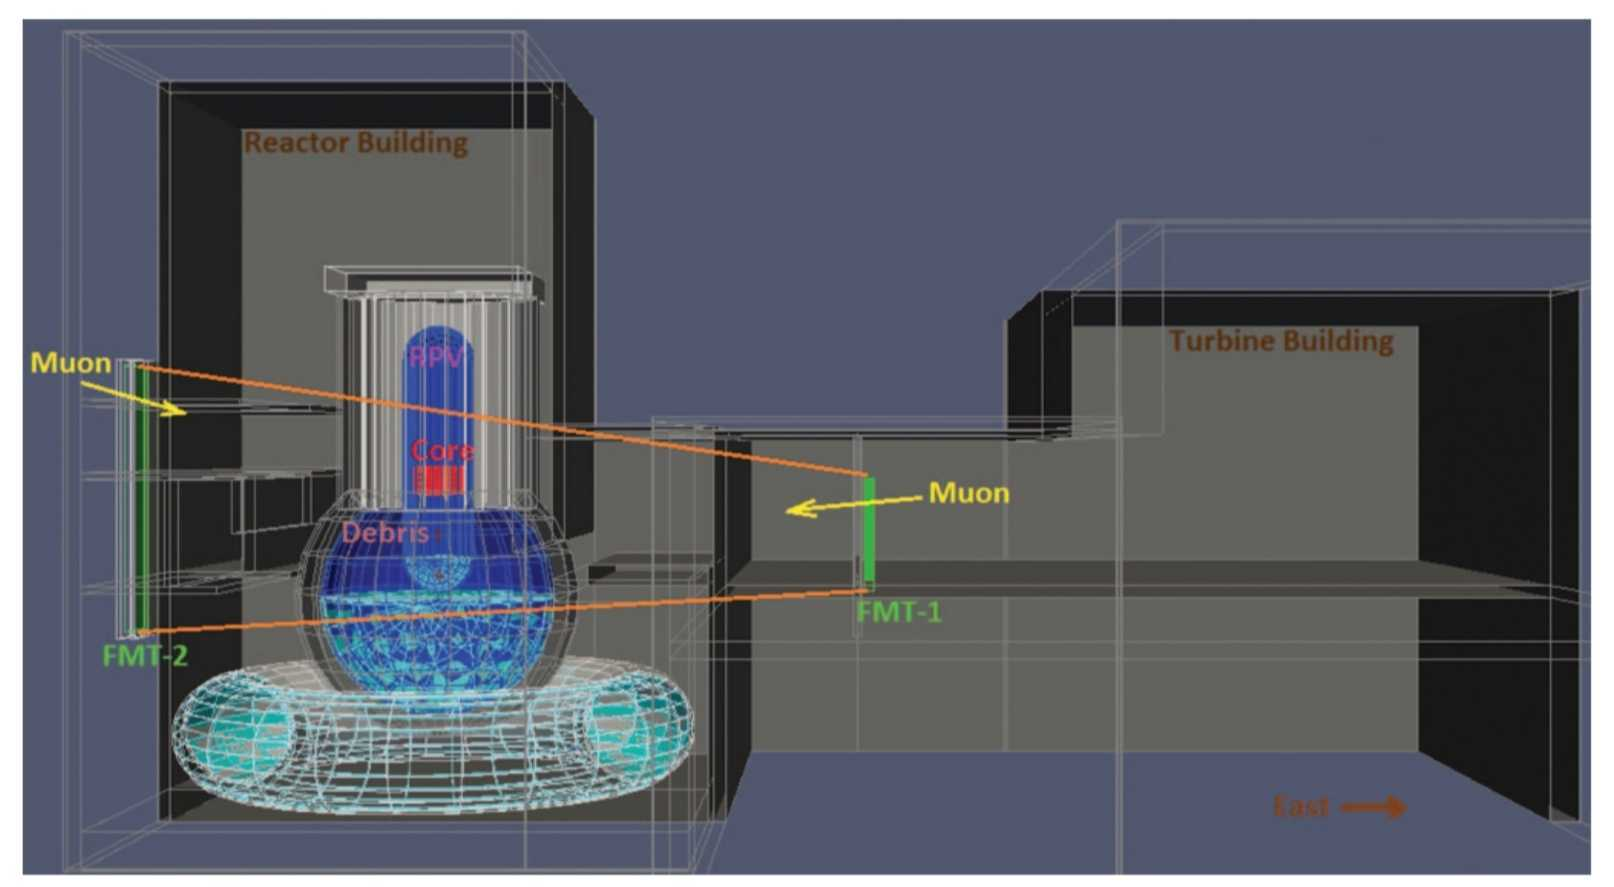
\includegraphics[width=0.7\linewidth]{Chapter5/Figs/MuTomographyExamples/fukushimaImaging.jpg}
 \captionof{figure}{$\mu$ imaging setup for Fukushima Unit 2. FMT-2 is installed inside a concrete radiation shield in front of the reactor building. $\mu$ scatting angles are a few degrees. From \cite{miyadera2013imaging}.} 
 \label{fig:fukushimaImaging}
\end{figure}

A result from the MMT is shown in figure \ref{fig:fukushimaFakeCore} where two-sided $\mu$ tomography is able to resolve a conical void similar in shape to the melted core of the Three Miles Island core. This lead core had two layers of concrete shielding blocks with a thickness of 2.74\,m each. Over a 3 week period 8 $\times$ 10$^4$ $\mu$ events were accumulated, this is an order of magnitude than what would be expected from the full deployment at Fukushima. 

\begin{figure}[!h]
 \centering
 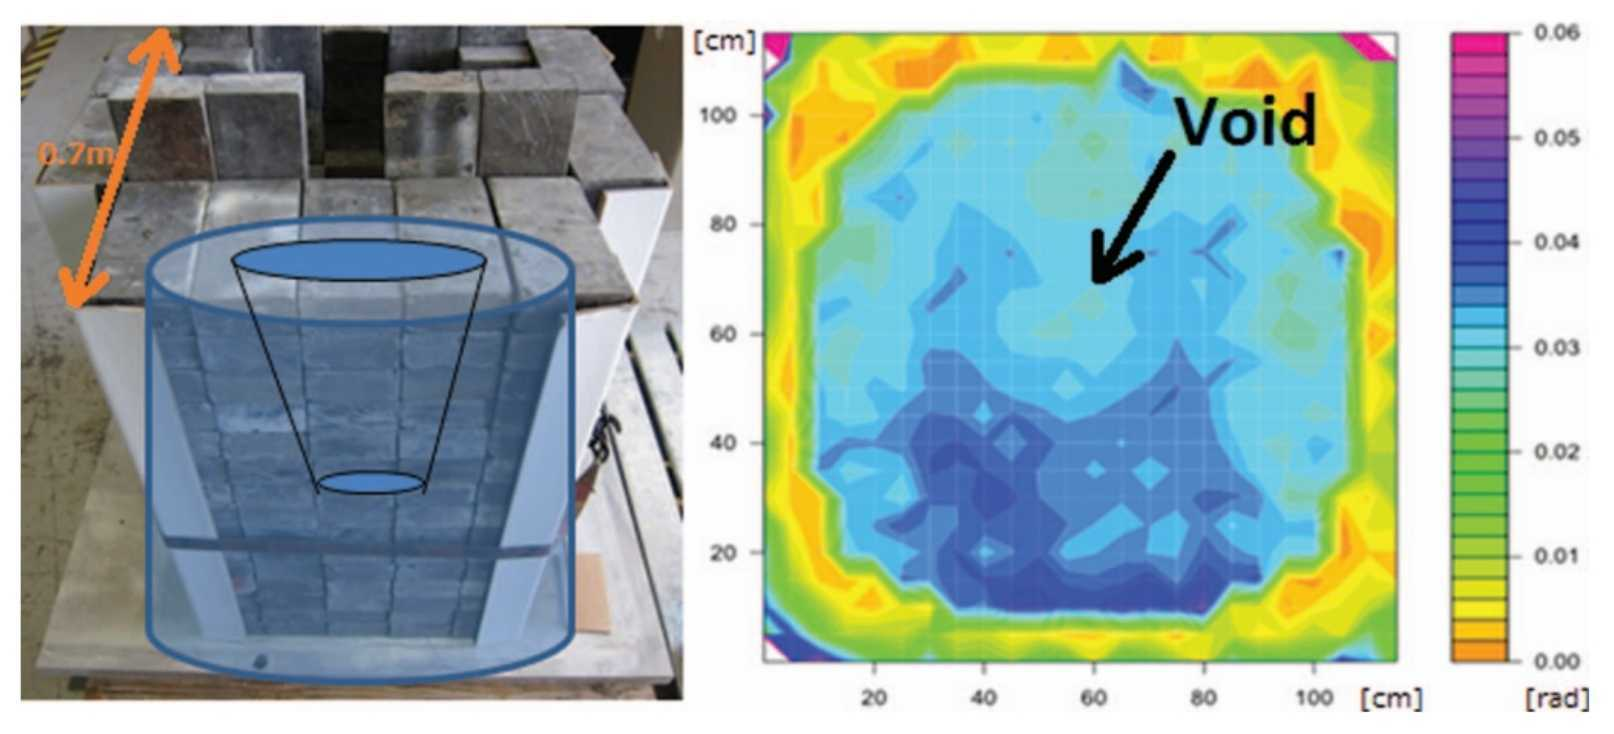
\includegraphics[width=0.7\linewidth]{Chapter5/Figs/MuTomographyExamples/FukushimaFakeCore.jpg}
 \captionof{figure}{Two-sided $\mu$ tomography of small example reactor core. Left -- Lead reactor core with conic void. Right -- observed core where average scattering angles of $\mu$ are plotted. The void in the core is clearly image through 2.74\,m concrete walls. Hot spots at the corners are artefacts caused by edge effects. From \cite{miyadera2013imaging}.} 
 \label{fig:fukushimaFakeCore}
\end{figure}
% Left -- Lead reactor core with conic void. Right -- observed core where average scattering angles of $\mu$ are plotted. The void in the core is clearly image through 2.74\,m concrete walls. The lead core of 0.7\,m thickness gives and equivalent radiation length to the uranium fuel in unit 1, and gives a similar scattering angle. Hot spots at the corners are artefacts caused by edge effects. From \cite{miyadera2013imaging}.

The MMT was then moved to the Toshiba facility at Kawasaki, Japan. The MMT was deployed for $\sim$ 4 weeks radiographing the Toshiba Critical Assembly Reactor using cosmic-ray $\mu$ \cite{morris2014analysis}. This was done to validate the concept of imaging the damaged cores at Fukushima Daiichi. The configuration for the Toshiba reactor can be seen in figure \ref{fig:Toshiba3dTomogarphy} and is similar to the proposed Fukushima setup. A comparison between GEANT4 Monte Carlo data is also shown in figure \ref{fig:toshibaG4Compare}. The quantitative agreement is within 3\,\% in measured density \cite{morris2014analysis}. These strong agreements show how powerful and predictable the results of two-sided cosmic $\mu$ tomography are, and why it is so often desired if an experiment can deploy multiple detectors and image a significant area. 

\begin{figure}[!h]
\centering
\begin{minipage}{.45\textwidth}
  \centering
  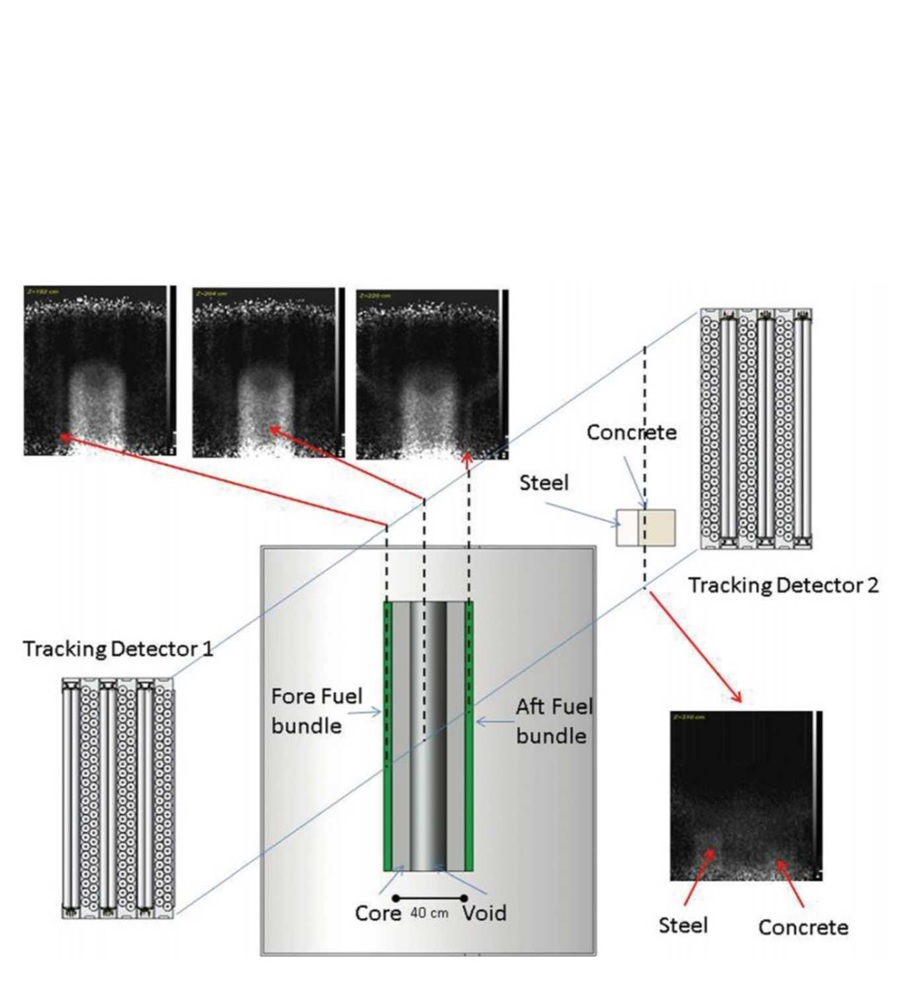
\includegraphics[width=\linewidth]{Chapter5/Figs/MuTomographyExamples/Toshiba3dTomogarphy.jpg}
  \captionof{figure}{Layout and some slices from the three dimension tomograph showing the major features in the Toshiba Nuclear Critical Assembly reactor image. From \cite{morris2014analysis}.} 
  \label{fig:Toshiba3dTomogarphy}
  \vspace{1.434cm} %1 line = 0.478cm % 2 lines = 0.956cm % 3 lines= 1.434cm % 4 lines = 1.912cm % 5 lines = 2.39cm
\end{minipage}%
\qquad
\begin{minipage}{.45\textwidth}
  \centering
  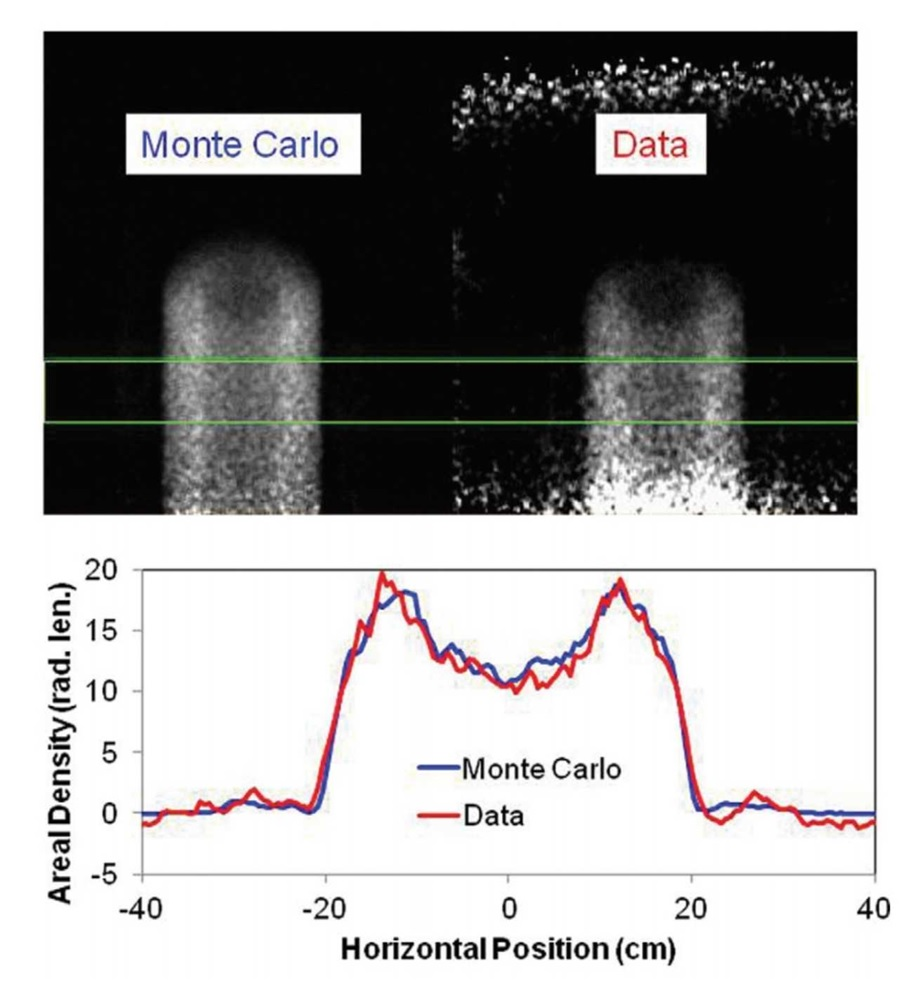
\includegraphics[width=\linewidth]{Chapter5/Figs/MuTomographyExamples/toshibaG4Compare.jpg}
  \captionof{figure}{GEANT4 Monte Carlo simulation vs. data for a slice through the centre of the Toshiba Nuclear Critical Assembly reactor core. Top images with the projected region marked by green lines. Bottom plots of the areal density vs. horizontal position. From \cite{morris2014analysis}.}
  \label{fig:toshibaG4Compare}
\end{minipage}
\end{figure}

% \begin{figure}[!h]
%  \centering
%  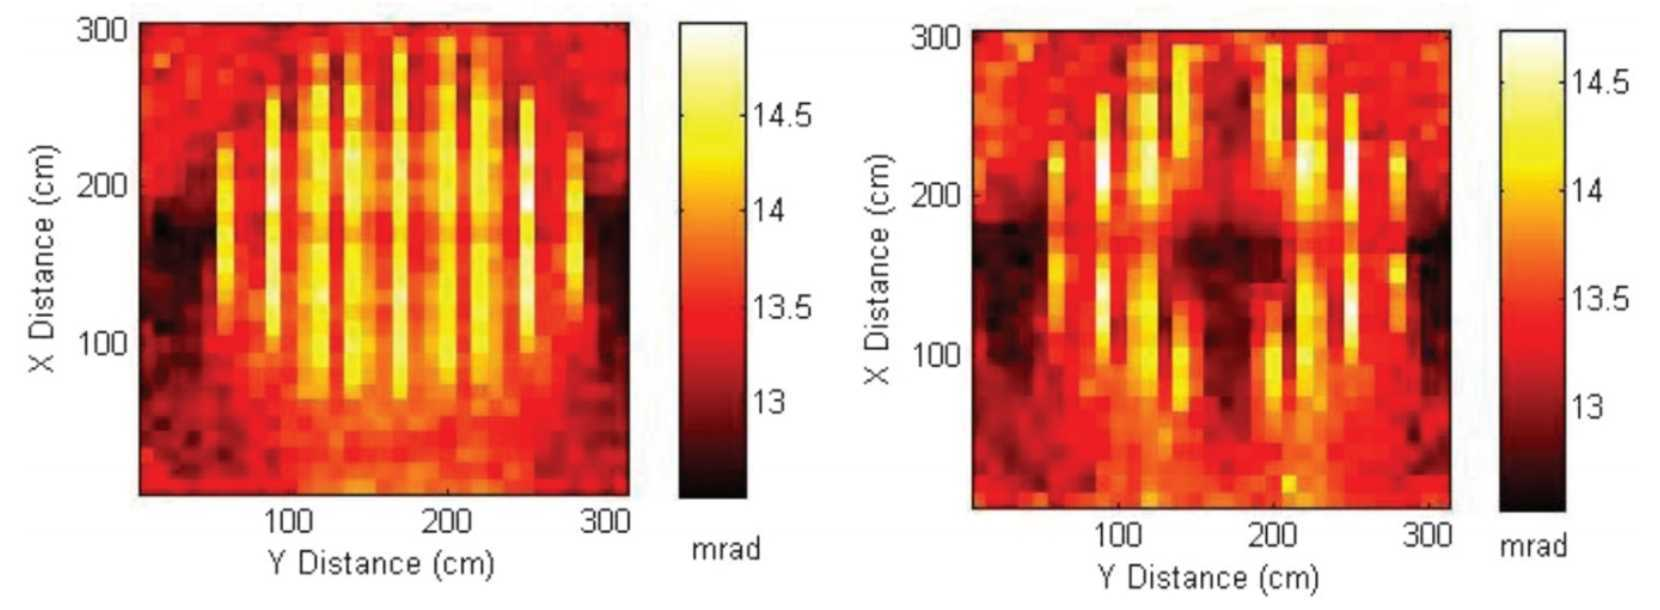
\includegraphics[width=1.0\linewidth]{Chapter5/Figs/MuTomographyExamples/2dZedCore.jpg}
%  \captionof{figure}{Reconstructed images of ZED-2 core during normal operating conditions (left) and a postulated accident scenario (right). Both images were reconstructed using two-sided muon tomography (see figure \ref{fig:Toshiba3dTomogarphy}). From \cite{Erlandson_reactorOST_2018}.} 
%  \label{fig:2dZedCore}
% \end{figure}

%\clearpage
\subsection{One-Sided Reactor $\mu$ Tomography}
% Open up with Canadian paper \cite{Erlandson_reactorOST_2018} 
% \\This reactor has already been imaged via two sided tomography
% \\Talk about benefits of portability and simplicity fig \ref{fig:Zed2Core1dRotation}, \cite{Fujii_ReactorRadiography_2019} 
% \\Then open up with radiography paper \cite{Fujii_ReactorRadiography_2019}
% \\Then mention the imaging of the reactor using one-sided tomography fig \ref{fig:JapcNuclearPowerImaging}, fig \ref{fig:JapcMt2Data} 
Whilst the benefits of two-sided tomography cannot be ignored there are distinct advantages to one-sided tomography. The comparative ease of deployment, ease of moving the detector or detector array, and multiple angles of measurement could allow for better tomography providing the correct approach is taken \cite{Erlandson_reactorOST_2018}. Unlike two-sided reactor tomography one-sided reactor tomography needs to be rotated around a reactor core to give a complete status of the core see figure \ref{fig:Zed2Core1dRotation} \cite{Erlandson_reactorOST_2018}. 

% \begin{figure}[!h]
%  \centering
%  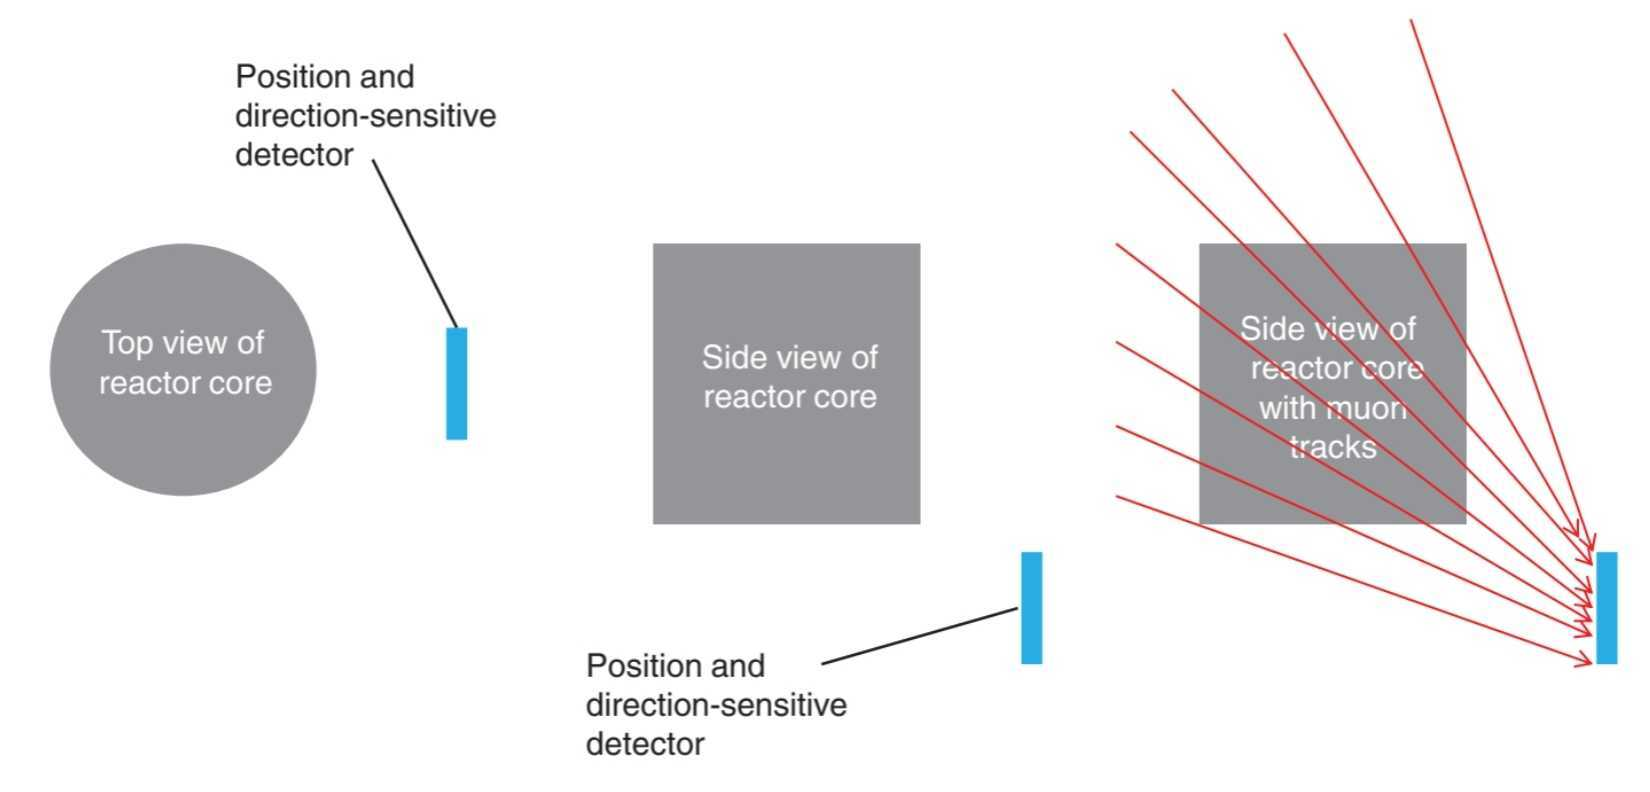
\includegraphics[width=0.8\linewidth]{Chapter5/Figs/MuTomographyExamples/ZdExplainationOf1D.jpg}
%  \captionof{figure}{Geometrical setup for the one-sided $\mu$ tomography concept.} 
%  \label{fig:ZdExplainationOf1D}
% \end{figure}

\begin{figure}[!h]
 \centering
 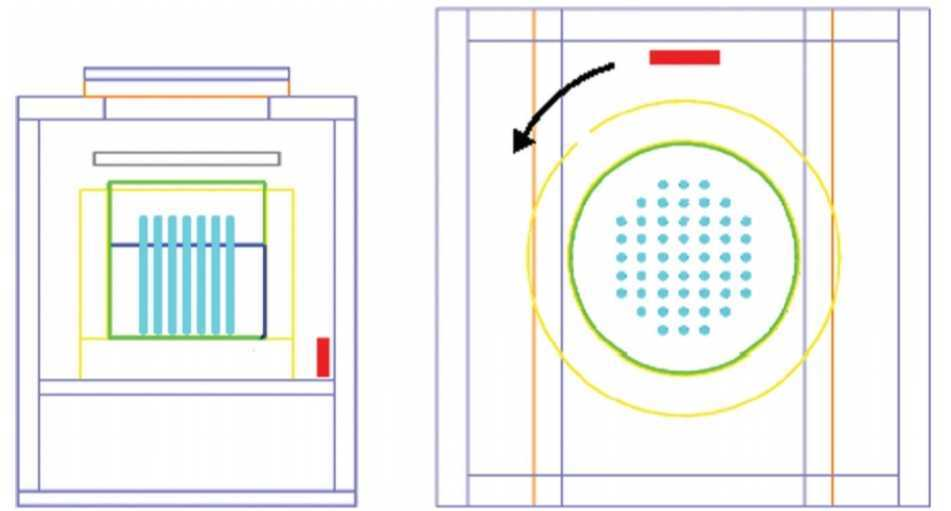
\includegraphics[width=0.7\linewidth]{Chapter5/Figs/MuTomographyExamples/Zed2Core1dRotation.jpg}
 \captionof{figure}{Detector placement for one-sided $\mu$ tomography of the ZED-D reactor. left: side-view. Right: top-view. From \cite{Erlandson_reactorOST_2018}.} 
 \label{fig:Zed2Core1dRotation}
\end{figure}

By simulating the ZED2 Canadian reactor core in GEANT4 Erlandson et al. were able to image the simulated core (see figure \ref{fig:Zed2OstSimulation}) \cite{Erlandson_reactorOST_2018} . The simulated reconstruction was done using the algebraic reconstruction technique (ART). This technique has 2 key inaccuracies seen in the middle row in figure \ref{fig:Zed2OstSimulation}. The first is the low density that has been reconstructed in the core. The second is the oscillating pattern of high density material where the fuel is present due to the 12 positions simulated for imaging the core\cite{Erlandson_reactorOST_2018} . These problems are overcome by taking a control data set before any damage and then subtracting that control distribution (left column of figure \ref{fig:Zed2OstSimulation}) from the ART results (middle row of figure \ref{fig:Zed2OstSimulation}) producing the bottom row of figure \ref{fig:Zed2OstSimulation} which clearly shows the damage in the core \cite{Erlandson_reactorOST_2018}. This technique requires more time ($\sim$ 33 days) than two-sided tomography ($\sim$ 5 days). But the size and cost of the required detectors is significantly greater then that of the proposed one-sided method \cite{Erlandson_reactorOST_2018}. This technique is of particular interest as rotating as rotating around a building to image it is very possible for VIDARR in a future deployment.

\begin{figure}[!h]
 \centering
 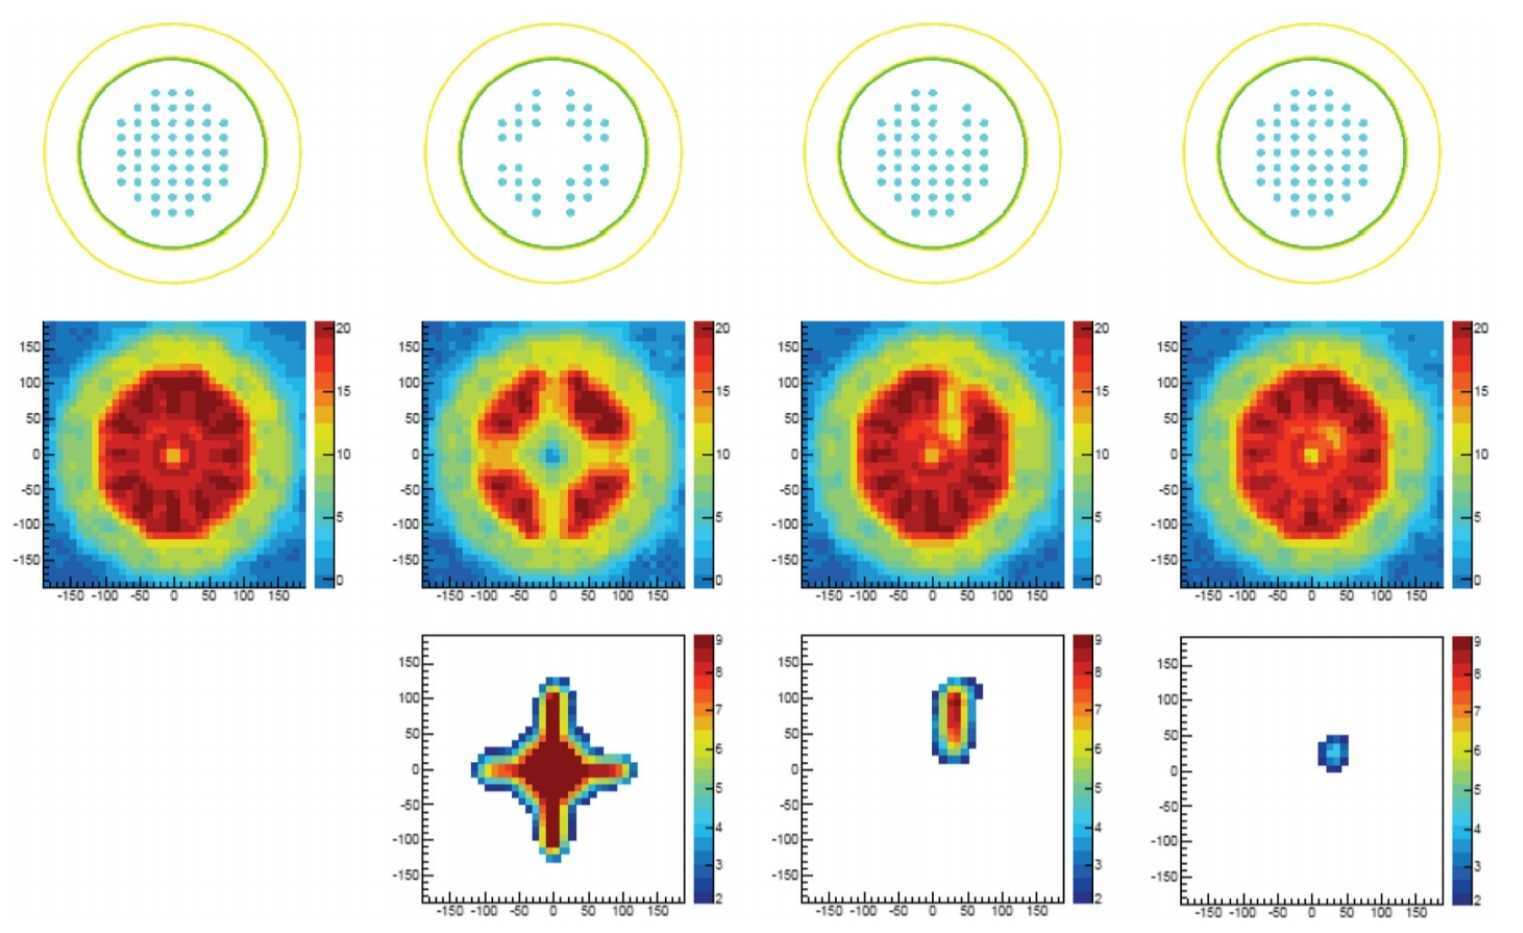
\includegraphics[width=1.0\linewidth]{Chapter5/Figs/MuTomographyExamples/Zed2OstSimulation.jpg}
 \captionof{figure}{Generated GEANT4 distributions for the ZED-2 research reactor. Top row: top-down projection of four different fuel channel configurations. Middle row: reconstructed images using 12 angles of detector and 1 iteration of the ART algorithm. Bottom row: background-subtracted images w in which the leftmost fuel configuration was used as the control case; the missing fuel is clearly visible in case. From \cite{Erlandson_reactorOST_2018}.} 
 \label{fig:Zed2OstSimulation}
\end{figure}

Imaging a reactor building from differing angles has already been done at the JAPC nuclear (see figure \ref{fig:JapcNuclearPowerImaging} and \ref{fig:3dImagingNFSP}). Even using thee positions (see figure \ref{fig:JapcNuclearPowerImaging}) it is possible to combine the detectors to image the nuclear fuel storage pond (NFSP) (see figure \ref{fig:3dImagingNFSP}) \cite{Fujii_ReactorRadiography_2019}. This successful 3d imaging shows a clear use for one-sided reactor $\mu$ tomography. The detectors were placed outside the reactor buildings, similar to VIDARR. By using three viewpoints the $\mu$ telescopes were able to observe the containment vessel, pressure vessel, and other components of the reactor building \cite{Fujii_ReactorRadiography_2019}. The three views also succeeded in locating two heavy object clusters which were considered to be the nuclear fuel assemblies stored in the NFSP (see figure \ref{fig:3dImagingNFSP}) \cite{Fujii_ReactorRadiography_2019}.

\begin{figure}[!h]
\centering
\begin{minipage}{.45\textwidth}
  \centering
  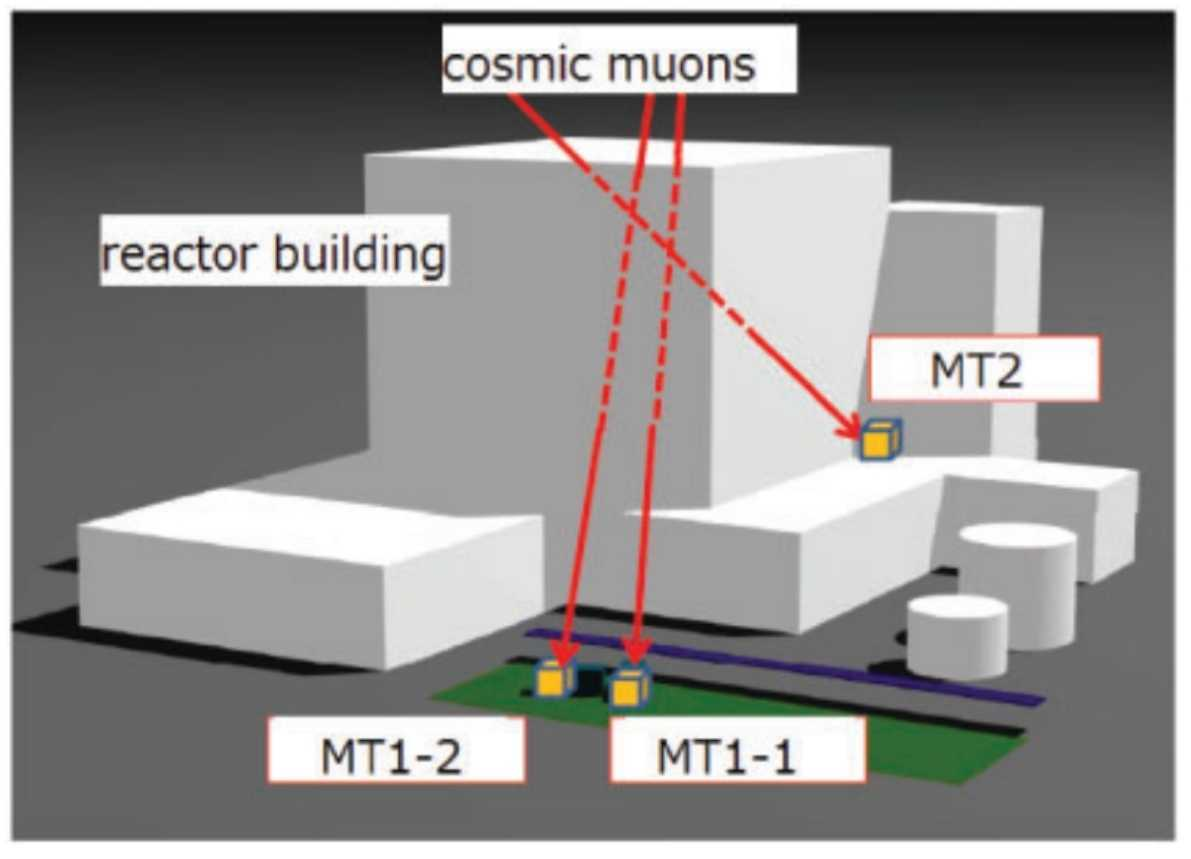
\includegraphics[width=\linewidth]{Chapter5/Figs/MuTomographyExamples/JapcNuclearPowerImaging.jpg}
  \captionof{figure}{Locations of the $\mu$ telescopes (marked as orange cubes) deployed at the JAPC nuclear power reactor. From \cite{Fujii_ReactorRadiography_2019}.} 
  \label{fig:JapcNuclearPowerImaging}
  \vspace{0.956cm} %1 line = 0.478cm % 2 lines = 0.956cm % 3 lines= 1.434cm % 4 lines = 1.912cm % 5 lines = 2.39cm
\end{minipage}%
\qquad
\begin{minipage}{.45\textwidth}
  \centering
  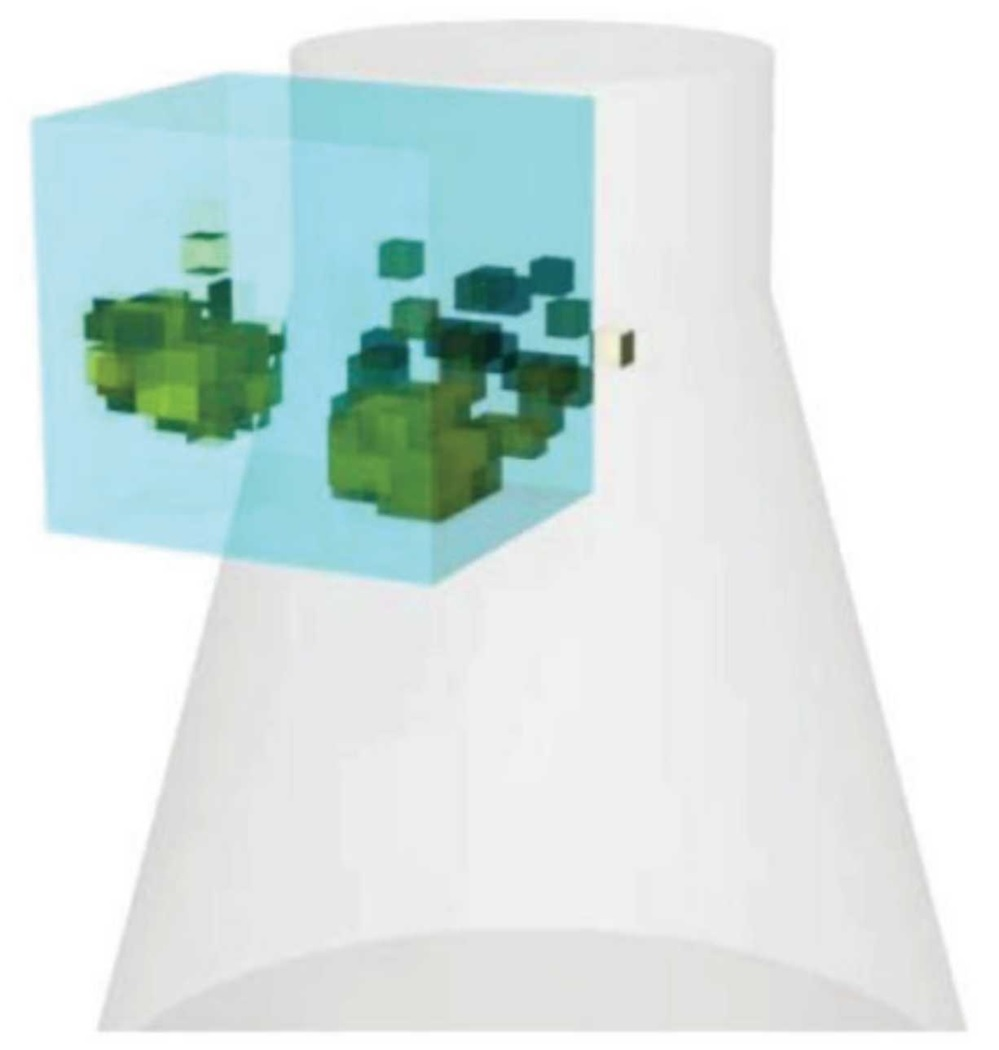
\includegraphics[width=\linewidth]{Chapter5/Figs/MuTomographyExamples/3dImagingNFSP.jpg}
  \captionof{figure}{A 3d image combined image from MT1, MT1-2, and MT2 deployed at JAPC nuclear power reactor. The blue area represents NFSP and the green blocks represent areas of high density i.e spent fuel. From \cite{Fujii_ReactorRadiography_2019}.}
  \label{fig:3dImagingNFSP}
\end{minipage}
\end{figure}

However, clear limitations of this technique are the time required and multiple deployments. VIDARR can be moved for specific purposes but ideally it should be deployed once and use $\mu$ tomography in a brief capacity for positional reconstruction. But this technique would still be possible with VIDARR producing the increased field of view is taken into account. But whether this is desirable will depend on the situations that the VIDARR detector is deployed under in the future. 

% \begin{figure}[!h]
%  \centering
%  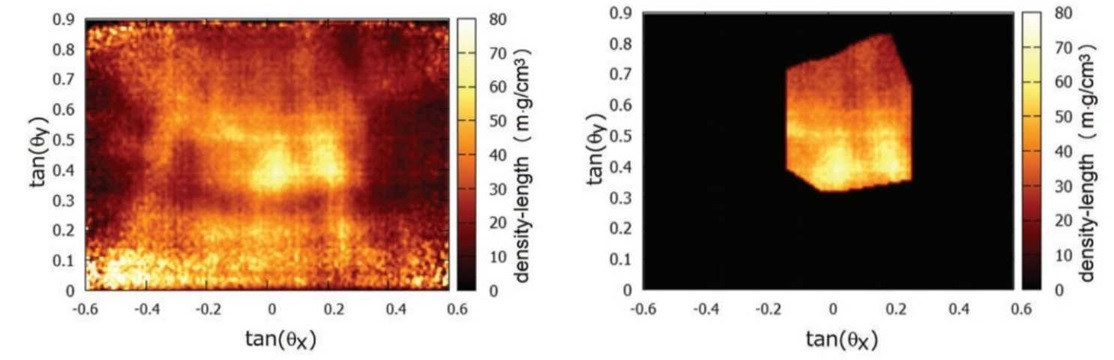
\includegraphics[width=1.0\linewidth]{Chapter5/Figs/MuTomographyExamples/JapcMt2Data.jpg}
%  \captionof{figure}{The density-length distributions estimated from MT2 data: (left) in the entire view area; (right) inside NFSP. From \cite{Fujii_ReactorRadiography_2019}.} 
%  \label{fig:JapcMt2Data}
% \end{figure}

% \begin{figure}[!h]
%  \centering
%  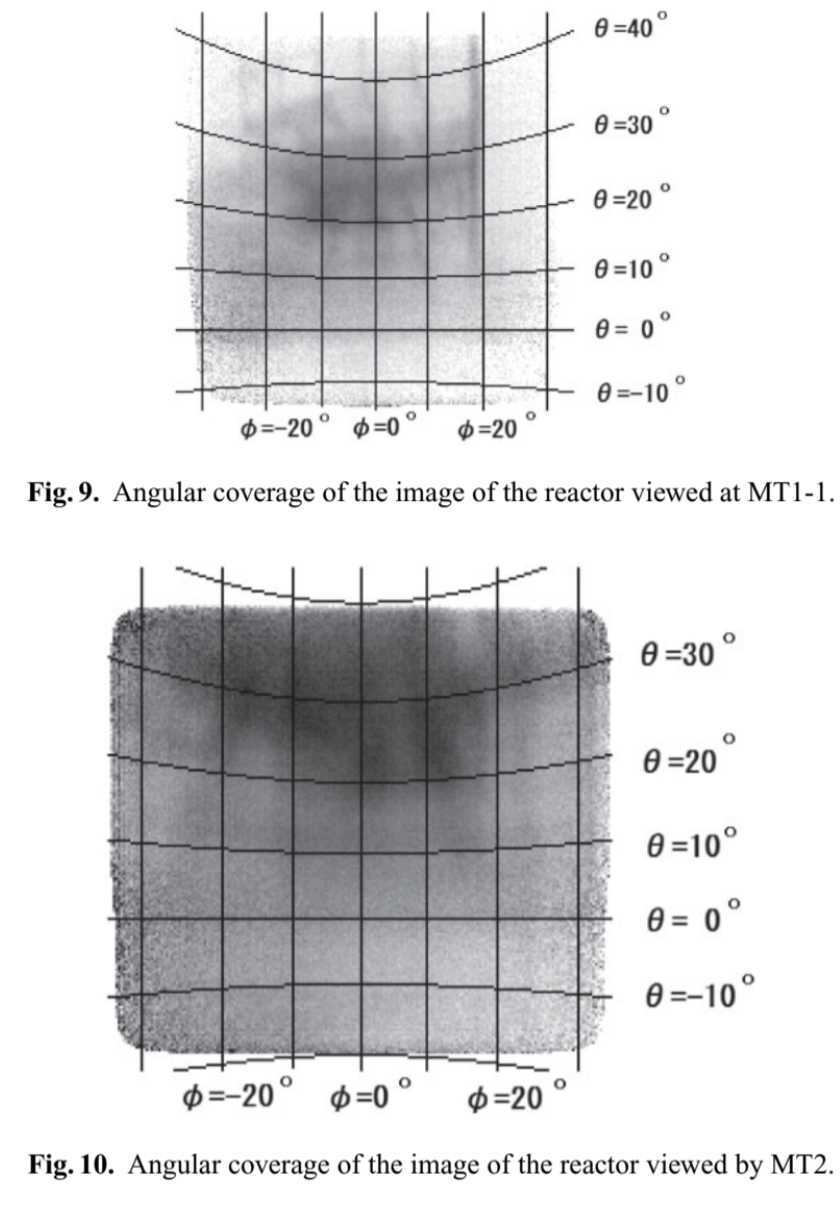
\includegraphics[width=1.0\linewidth]{Chapter5/Figs/MuTomographyExamples/JapcImagingCovering.jpg}
%  \captionof{figure}{.} 
%  \label{fig:JapcImagingCovering}
% \end{figure}

% \subsection{Mt. Asama Imaging}
\subsection{Geological One-Sided $\mu$ Tomography}  \label{sec:geologicalTomography} %\label{sec:DIAPHANEmuRadiography}
% One sided 3-d tomography of a volcano fig \ref{fig:mtAsma3dMap}, \cite{Tanaka_mtAsama_2007} 
% \\Muon radiography 
% \\one distant detector fig \ref{fig:MtAsma1dExplanation}
Geological $\mu$ tomography relies on imaging large objects, typically volcanoes. This is very similar to imaging a distant reactor buildings with VIDARR. For example, in 2007 Mt.Asama in Japan was successfully imaged using an emulsion-cloud-chamber. This distant detector was able to image on coming $\mu$ traversing through the mountain (see figure \ref{fig:MtAsma1dExplanation}) \cite{Tanaka_mtAsama_2007}. Through the use of $\mu$ radiography (determining how much energy the traversing $\mu$ particles have lost) an accurate top down map of rock densities can be produced (see figure \ref{fig:mtAsma3dMap}) \cite{Tanaka_mtAsama_2007}. This top down tomographic map is impressive, as it requires the correlation of map data and cosmic $\mu$ data. VIDARR should be capable of this too but the time requirement is likely too large for VIDARR to produce such a map. 

\begin{figure}[!h]
\centering
\begin{minipage}{.45\textwidth}
  \centering
  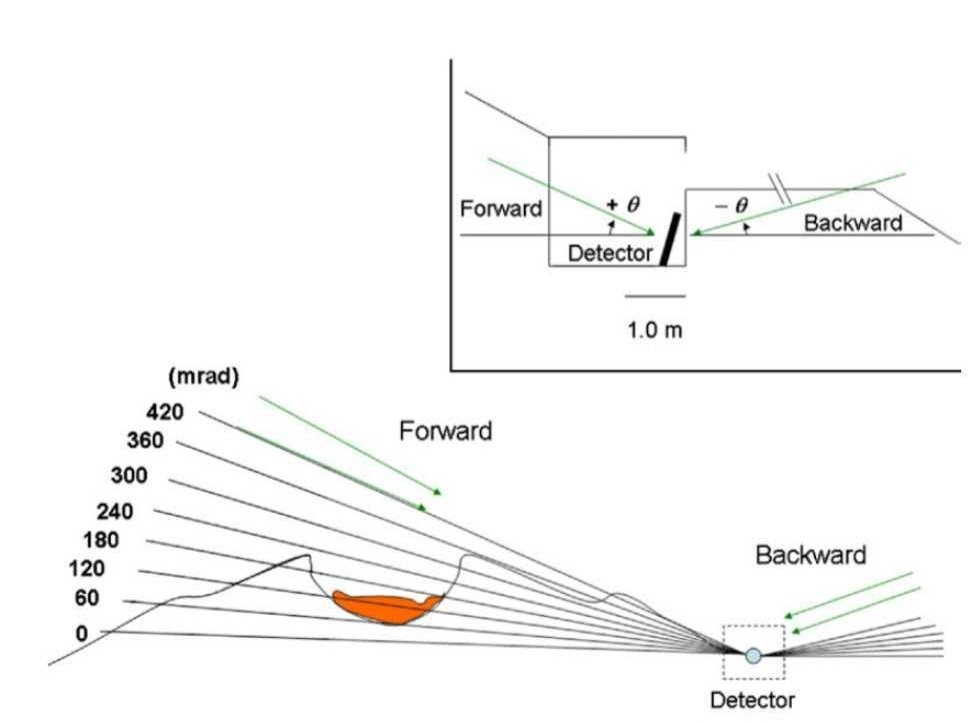
\includegraphics[width=\linewidth]{Chapter5/Figs/MuTomographyExamples/MtAsma1dExplanation.jpg}
  \captionof{figure}{Cross-section of Mt. Asama showing geometrical arrangements used in the present measurements. The data or $\mu$ arriving from the backward direction are also used to confirm the detector efficiency. The inset shows the detector arrangements in the underground space. From \cite{Tanaka_mtAsama_2007}.} 
  \label{fig:MtAsma1dExplanation}
  \vspace{2.39cm}%5 lines = 2.39cm
\end{minipage}%
\qquad
\begin{minipage}{.45\textwidth}
  \centering
  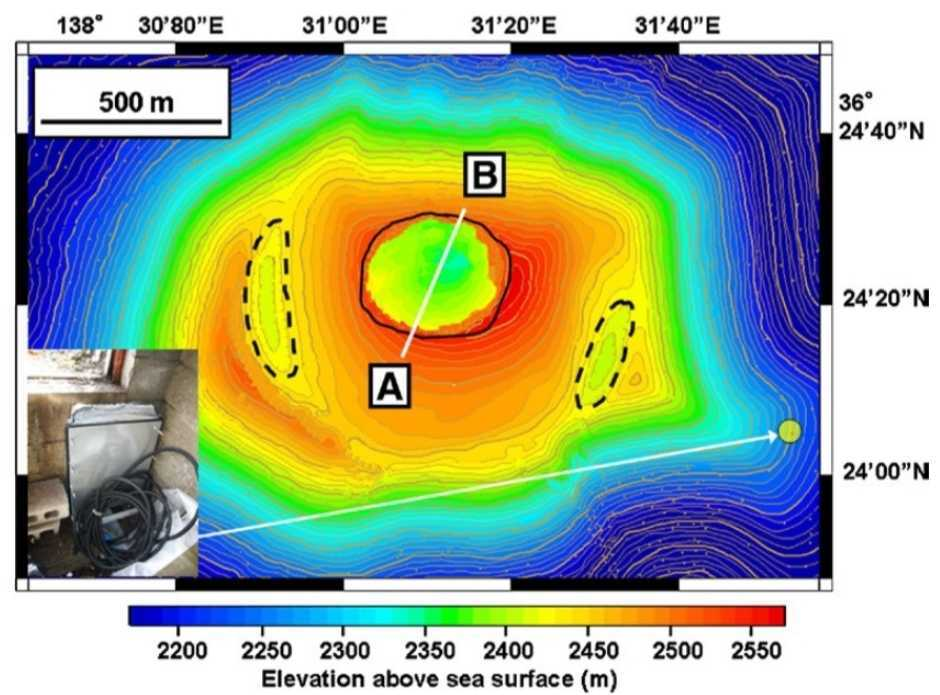
\includegraphics[width=\linewidth]{Chapter5/Figs/MuTomographyExamples/mtAsma3dMap.jpg}
  \captionof{figure}{Map of Mt.Asama showing the location of the cosmic-ray $\mu$ detector (arrow). Inset is a photograph showing the emulsion-cloud-chamber cosmic-ray $\mu$ detector made of iron plates and nuclear emulsion films. The white solid line A--B, parallel to the horizontal edge of the detector, shows the vertical cross-sectional plane of the crater. The old crater (dotted lack lines) of Mt. Maekake-yama has been buried with a new pyroclastic cone (Mt. Kama-yama) with a summit crater (solid black line).}
  \label{fig:mtAsma3dMap}
\end{minipage}
\end{figure}

The DIAPHANE detector is a plastic scintillating detector with bars with WLS fibres threaded down the centre similar to VIDARR. Instead of using silicon photomultipliers the DIAPHANE detector uses multianode PMT’s to read out the light from the WLS fibres \cite{Marteau_2017}. The DIAPHANE telescope seen in figure \ref{fig:DIAPHANE_deployment} is a series of 3 planes on a rotating platform with adjustable height. Each plane in DIAPHANE consists of two layers rotated at 90$^\circ$ to each other. The bars in each layer have a rectangular cross section of 5\,cm $\times$ 1\,cm \cite{MARTEAU201223}. 
% Both DIAPHANE and MU-RAY have taken tomographic data to image their surroundings. With DIAPHANE imaging La Soufriere of Guadeloupe using cosmic $\mu$ radiography as seen in figure \ref{fig:diaphaneStructualImaging} which shows the different density areas of rock relevant for volcanology \cite{Marteau_2017}.  MU-RAY has also produced similar results for mt. Vesuvius in figure \ref{fig:mtVesuviusMuRayImaging}. Though their technique and data only provide results of rock thickness in meters rather than density \cite{Ambrosino_2014}. Of more interest is figure \ref{fig:mtVesuviusMuRayTransmission} from MU-RAY which shows the ``Transmission'' method. The transmission method used in figure \ref{fig:mtVesuviusMuRayTransmission} is obtained by pointing the MU-RAY detector at the sky for a calibration period of one week then pointing the MU-RAY detector at Mt Vesuvius for one week and then taking the ratio of the two data sets \cite{Ambrosino_2014}. This approach of measuring the free sky and the blocked sky and taking the ratio of the two creates an extremely clear image because it takes the background into account. This creates a clear difference in intensity where transmission of 1 represents the free sky and transmission of 0 represents completely blocked sky. This approach is the one that will be used when analysing the Wylfa reactor site (see chapter \ref{chp:cosmicMuonTomography}) due to the effective reduction of background noise effects and the sharpness of the image it provides. 
% \\\\The DIAPHANE experimental setup seen in figure \ref{fig:DIAPHANE_deployment} shows a cosmic $\mu$ telescope with several different planes clearly analysing a very narrow field of view this helps significantly in preventing distortions via bin migration. This is also the case for the MU-RAY collaboration as seen in figure \ref{fig:muRayDetectors} the detector is also multiple flat planes. Each plane in MU-RAY is compromised of triangular prisms with WLS fibres running down the middle (see figure \ref{fig:muRaySetup}). Both MU-RAY and DIAPHANE are traditional cosmic $\mu$ telescopes as opposed to VIDARR which is an $\Bar{\nu_e}$ detector first and a cosmic $\mu$ camera second. Despite this DIAPHANE, MU-RAY, and VIDARR all use similar technology: plastic scintillating bars and WLS fibres \cite{Carroll_2018} \cite{Marteau_2017} \cite{ANASTASIO2013423}. DIAPHANE uses ``multianode PMT’s'' to read out information from the WLS fibres \cite{Marteau_2017} whereas VIDARR and MU-RAY use SiPms \cite{Carroll_2018} \cite{ANASTASIO2013423} to read out the information from the WLS fibres. 

\begin{figure}[!h]
 \centering
 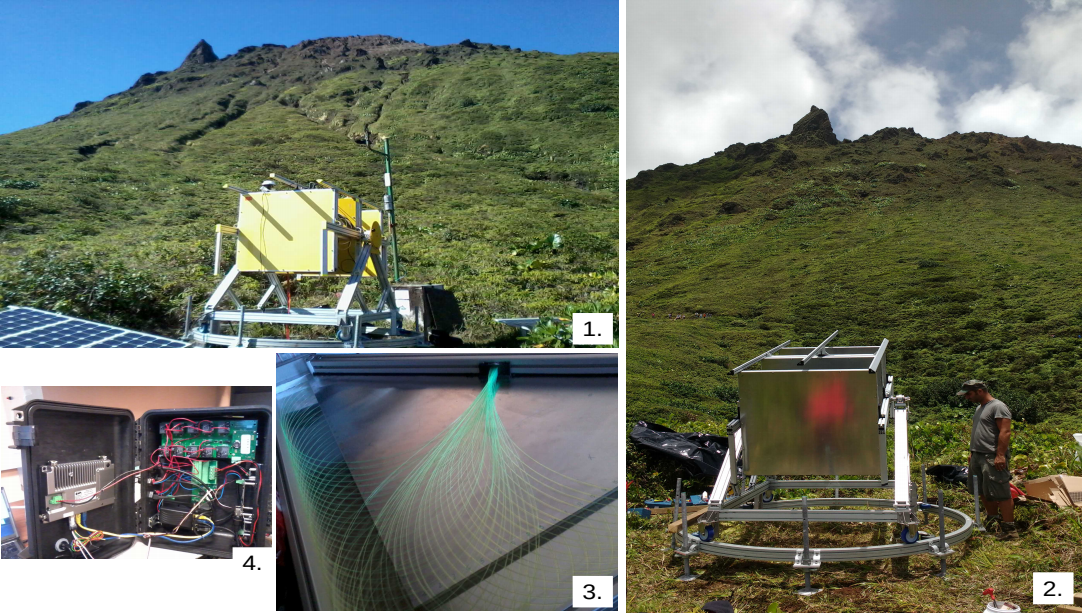
\includegraphics[width=1.0\linewidth]{Chapter5/Figs/Raster/DIAPHANE_deployment.png}
 \captionof{figure}{The deployment of the DIAPHANE detector from \cite{Marteau_2017}. DIAPHANE $\mu$ detectors upgrades. 1: the first generation 3 planes $\mu$ detector on the slope of La Soufrière of Guadeloupe (PK site). 2: the second-generation 3 planes $\mu$ detector, with a transverse segmentation divided by a factor 2, on the slope of La Soufrière of Guadeloupe (SAM site). 3: inner WLS fibres collected on a PMT cookie. 4: compact CTRL BOX with embedded hardened processing unit and electronics: common clock signal, WebRelay, Ethernet switch, Power-over-Ethernet to the wifi antenna. From \cite{Marteau_2017}.} 
 \label{fig:DIAPHANE_deployment}
\end{figure}

The DIAPHANE detectors are used to image the slope of La Soufrière of Guadeloupe. A volcano of interest. Through use of cosmic $\mu$ radiography the goal of DIAPHANE is to image the interior structure of the volcano by determining the density of the rock at Guadeloupe. This technique requires a significant amount of time to obtain sufficient clarity. DIAPHANE was deployed between 2010 -- 2016 in which the experiment was able to produce the results seen in figure \ref{fig:diaphaneStructualImaging}. Whilst these results are impressive and give a highly detailed reconstruction the time frame to achieve these results is very long. For VIDARR this technique would would not be suitable as a time scale for cosmic $\mu$ tomography will be $\sim$ 1 hour. However, due to the similar size and shape of the segments between DIAPHANE and VIDARR it's reasonable to conclude that the segmentation effects can be worked around to produce clear images. 

\begin{figure}[!h]
 \centering
 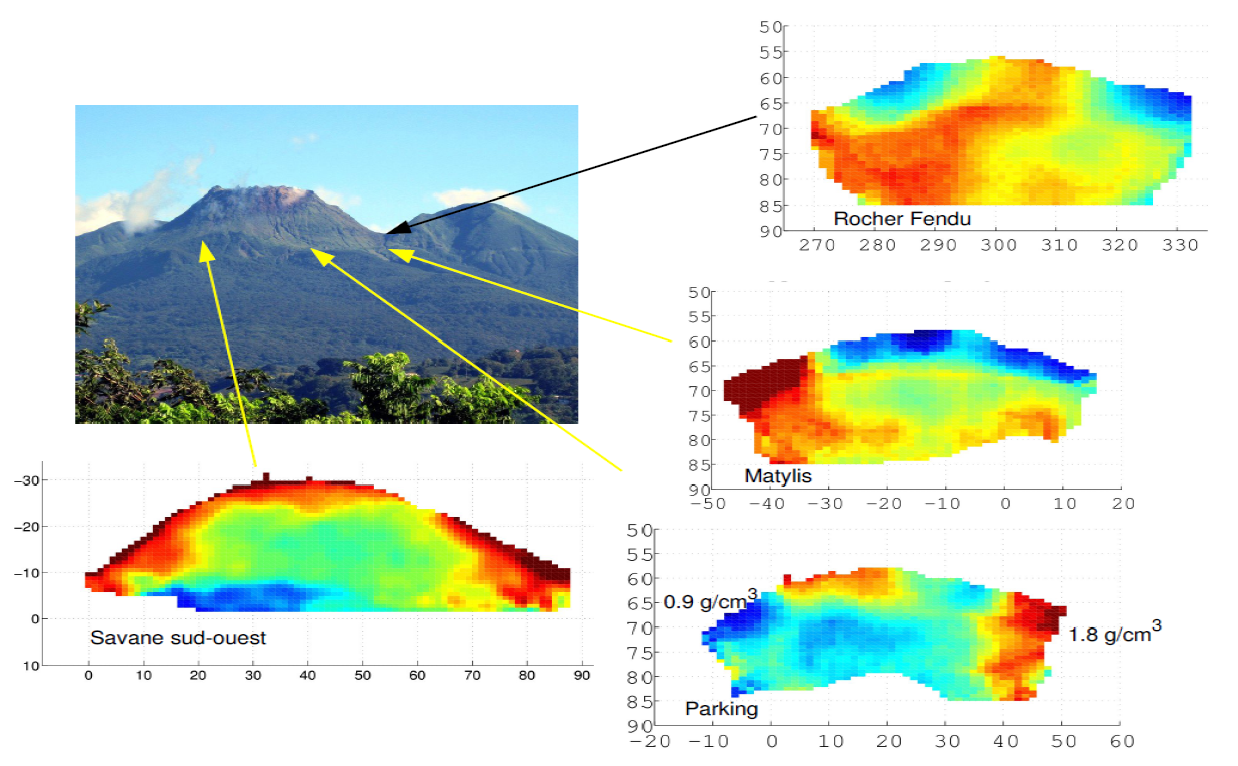
\includegraphics[width=1.0\linewidth]{Chapter5/Figs/Raster/diaphane_structuralImaging.png}
 \captionof{figure}{DIAPHANE structural imaging of the La Soufrière of Guadeloupe dome from 4 different acquisition sites around the dome. The blue areas are the less dense zones of the volcano. The red areas have the highest density. The average density extracted from all those images ranges from 1.6 to 1.8 g.cm$^{-3}$. From \cite{Marteau_2017}} 
 \label{fig:diaphaneStructualImaging}
\end{figure}

% \subsection{MU-RAY Tomography and Transmission Method} \label{sec:murayTomographyAndTransmissionMethod}
The MU-RAY collaboration also uses cosmic $\mu$ radiography to analyse Mt.Vesuvius. The detector uses plastic scintillator and silicon photon multipliers (SiPms) similar to that of VIDARR \cite{ANASTASIO2013423} \cite{Ambrosino_2014}. Apart from the scintillator shape which is the shape of a triangular prism in MU-RAY and the shape of a cuboid in VIDARR the two use very similar technology. The experimental setup is very similar to that of DIAPHANE with panels arranged with regular intervals (see Figure \ref{fig:muRayDetectors}). The goals of DIAPHANE and MU-RAY are the same -- to image the interior of volcanoes. MU-RAY even has low power requirements hence solar panels can be used for power in remote locations \cite{ANASTASIO2013423}. 

% \begin{figure}[!h]
%  \centering
%  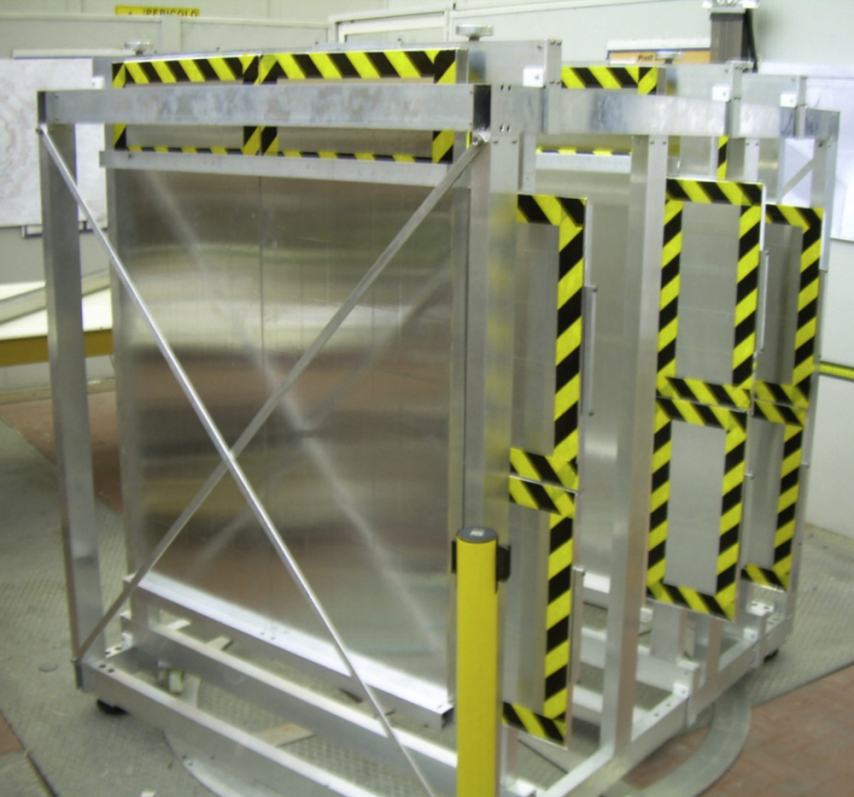
\includegraphics[width=0.5\linewidth]{Chapter5/Figs/Raster/muRayDetectors.png}
%  \captionof{figure}{The MU-RAY detector frame with the three X–Y planes mounted. The frame can be oriented using the rotating platform visible at the bottom. From \cite{ANASTASIO2013423}} 
%  \label{fig:muRayDetectors}
% \end{figure}

The limits of $\mu$ radiography is clearly demonstrated by figure \ref{fig:mtVesuviusMuRayImaging}. Whilst the MU-RAY detector was deployed with no obstructions and had a deployment time of $\sim$ 1 month and was elevated by 800\,m reducing atmospheric scattering the outline of Mt.Vesuvius is still faint. Whilst the increase in rock thickness is clearly visible in figure \ref{fig:mtVesuviusMuRayImaging} there are no clear defining features. These results are in stark contrast to the DIAPHANE results at Guadeloupe (figure \ref{fig:diaphaneStructualImaging}) which show clear interior structural imaging of a volcano. Whilst the technology of DIAPHANE and MU-RAY is not identical they are very similar. DIAPHANE has better energy reconstruction due to the multianode PMT’s as opposed to the SiPms used in MU-RAY \cite{Marteau_2017}, \cite{ANASTASIO2013423}. However, the spatial reconstruction should be superior in MU-RAY as the segments in DIAPHANE have a cross section of 5\,cm $\times$ 1\,cm (5\,cm$^2$) \cite{MARTEAU201223}, whereas the MU-RAY triangular cross section has a base width of 3.3\,cm and height 1.7\,cm (2.805\,cm$^2$). As a result the blurry resolution in figure \ref{fig:mtVesuviusMuRayImaging} is surprising and leads to the conclusion that the 5 year deployment time for DIAPHANE is the main reason for the sharper resolution in figure \ref{fig:diaphaneStructualImaging}.

\begin{figure}[!h]
\centering
\begin{minipage}{.45\textwidth}
  \centering
  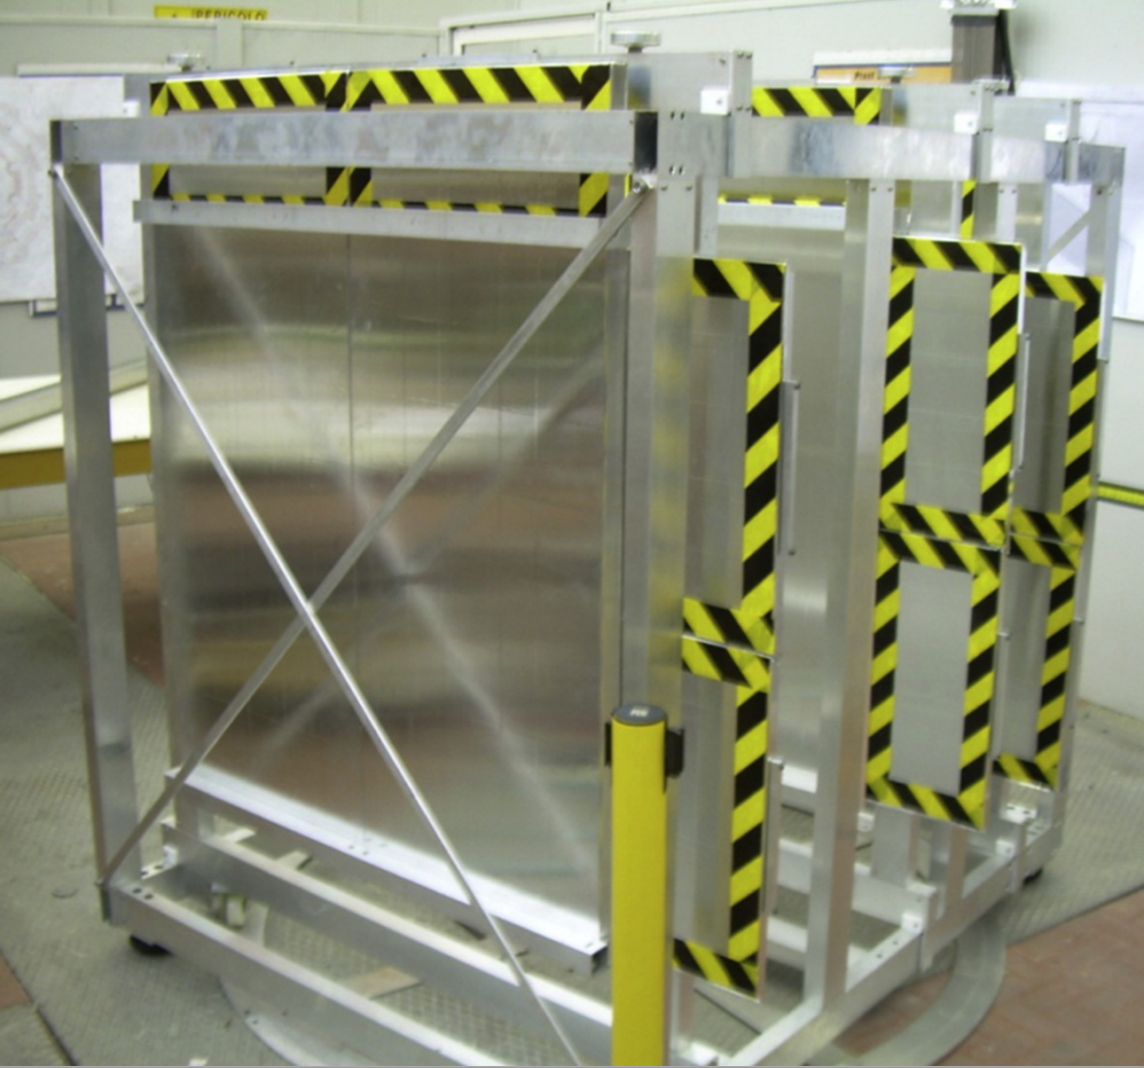
\includegraphics[width=\linewidth]{Chapter6/Figs/Raster/muRayDetectorsAdj.png}
  \captionof{figure}{The MU-RAY detector frame with the three X–Y planes mounted. The frame can be oriented using the rotating platform visible at the bottom. From \cite{ANASTASIO2013423}.} 
  \label{fig:muRayDetectors}
  \vspace{0.478cm} %1 line = 0.478cm % 2 lines = 0.956cm % 3 lines= 1.434cm % 4 lines = 1.912cm % 5 lines = 2.39cm
\end{minipage}%
\qquad
\begin{minipage}{.45\textwidth}
  \centering
  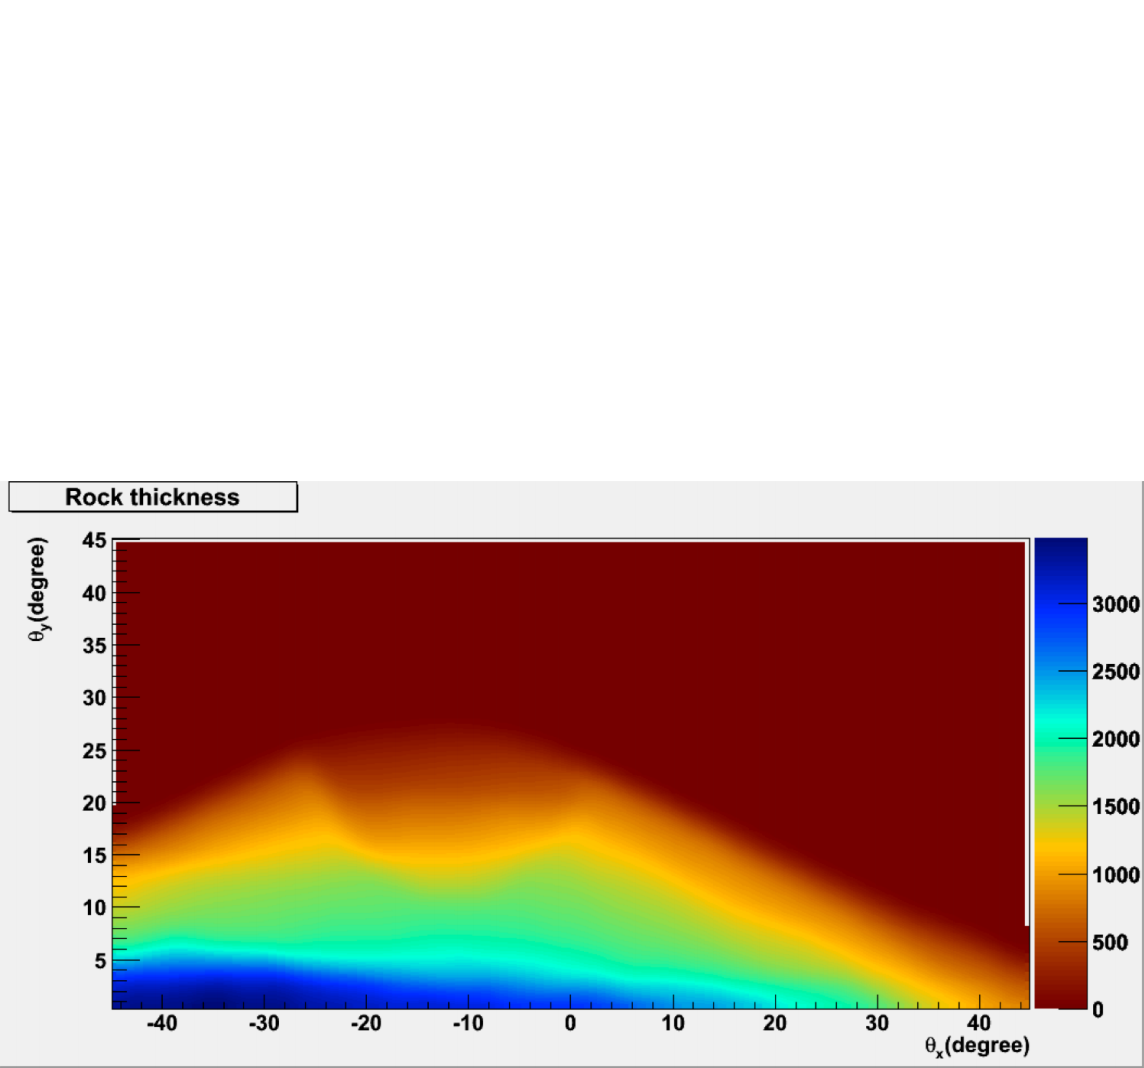
\includegraphics[width=\linewidth]{Chapter6/Figs/Raster/mtVesuviusMuRayImagingAdj.png}
  \captionof{figure}{MU-RAY telescope analysing Vesuvius rock thickness, expressed in m, as seen from the observation point at $\sim$ 800\,m altitude. With data taken over a month period of $\sim$ 1 month. From \cite{Ambrosino_2014}.}
  \label{fig:mtVesuviusMuRayImaging}
\end{minipage}
\end{figure}

As a result of their limited deployment time the MU-RAY collaboration took $\sim$ 1 week to image Mt.Vesuvius using a different technique. The transmission technique. The results are shown in figure \ref{fig:mtVesuviusMuRayTransmission} whilst this data set has $\sim$ 4 times live time data than for figure \ref{fig:mtVesuviusMuRayImaging} the results are much clearer. The transmission method takes the ratio of the unblocked vertical sky with the area where Mt.Vesuvius is located \cite{Ambrosino_2014}. The effect is so significant because the acceptance and efficiency dependencies are cancelled out as such when normalised to the acquisition run the free sky zone common to both histograms should be close to 1 \cite{Ambrosino_2014}. This is especially useful for cosmic $\mu$ tomography for VIDARR as the field of view is much wider.

% \begin{figure}[!h]
%  \centering
%  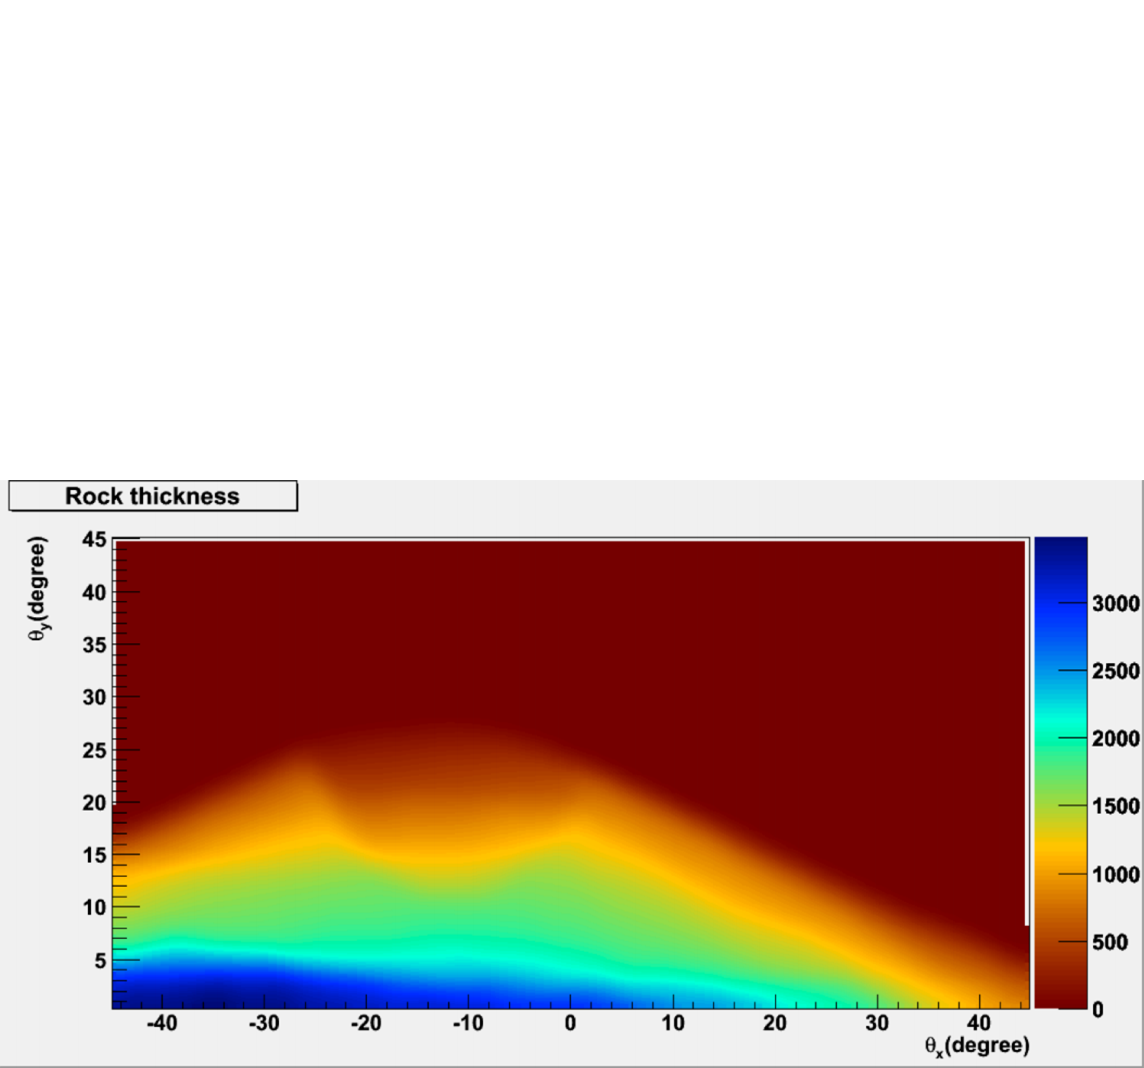
\includegraphics[width=0.6\linewidth]{Chapter5/Figs/Raster/mtVesuviusMuRayImaging.png}
%  \captionof{figure}{MU-RAY telescope analysing Vesuvius rock thickness, expressed in m, as seen from the observation point at $\sim$ 800\,m altitude. With data taken over a month period of $\sim$ 1 month. From \cite{Ambrosino_2014}.} 
%  \label{fig:mtVesuviusMuRayImaging}
% \end{figure}

\begin{figure}[!h]
 \centering
 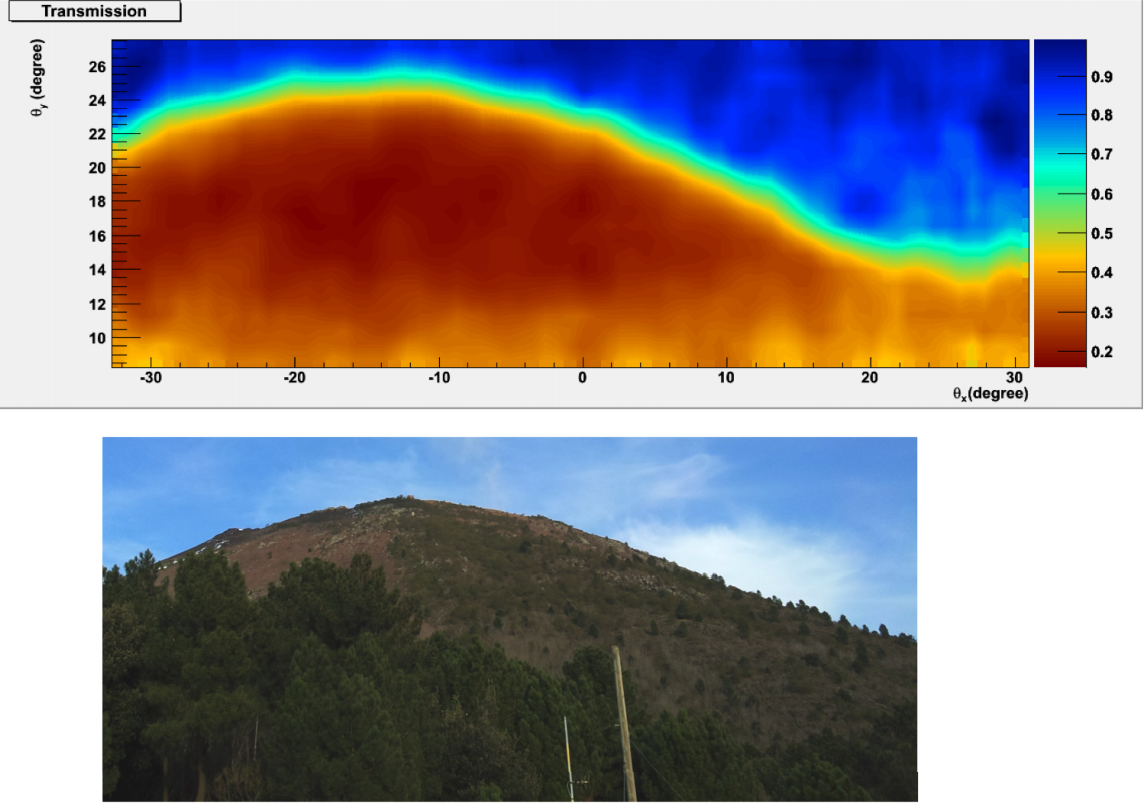
\includegraphics[width=0.8\linewidth]{Chapter5/Figs/Raster/mtVesuviusMuRayTransmission.png}
 \captionof{figure}{MU-RAY data from Vesuvius. Top: the transmission histogram of Mt Vesuvius after one week of data taking. Bottom: a picture of Mt Vesuvius taken by the telescope observation point. Taken over a period of $\sim$ 1 week. From  \cite{Ambrosino_2014}.} 
 \label{fig:mtVesuviusMuRayTransmission}
\end{figure}
